\documentclass[11pt]{report}
\usepackage[paper=a4paper,margin=2.5cm]{geometry}
\usepackage[outputdir=out]{minted}
\usepackage{multicol}
\usepackage{fontspec}

% Point fontspec at your local fonts folder:
\setmainfont{EBGaramon}[
  Path      = font/,       % relative to main.tex
  Extension = .ttf,
  UprightFont    = *d12-Regular,   % MyFont-Regular.ttf
  BoldFont       = *d08-Regular,       % MyFont-Bold.ttf
  ItalicFont     = *d12-Italic,
  BoldItalicFont = *d08-Italic
]

\usepackage{forest}
\usepackage{microtype}
\usepackage{graphicx}
\usepackage{wrapfig}
\usepackage[colorlinks,linkcolor=blue,urlcolor=cyan]{hyperref}
\usepackage{titlesec}
\titleformat{\chapter}[hang]{\normalfont\huge\bfseries}{}{0pt}{}
\titlespacing*{\chapter}{0pt}{1.5em}{1em}
%=== Metadata ===
\newcommand{\thesistitle}{Your Thesis Title Here}
\newcommand{\authorname}{Rafael Tanzer}
\newcommand{\supervisor}{Michele Chiaria, Simone , Francesco Pontigia and Ezzio Bartocci}
\newcommand{\institution}{TU Vienna}
\newcommand{\department}{Cyber-Physical-Systems, ..., ...}
\newcommand{\logoimage}{graphics/logo.png} % Path to your logo image
\newcommand{\submissionmonth}{May}
\newcommand{\submissionyear}{2025}
%================

\usepackage[backend=biber, style=numeric]{biblatex}
\addbibresource{bibliography/theory.bib}
\addbibresource{bibliography/implementation.bib}
\usepackage{./simplebnf}
\def\code#1{\texttt{#1}}

\begin{document}

\begin{titlepage}
  \centering
  \vspace*{1cm}

  % University logo
  
\includegraphics[width=0.25\textwidth]{graphics/tuWienLogo.png}
  \\[1cm]

  % Thesis title
  {\Huge \thesistitle\\[1.5cm]}

  % Project logo under title, smaller size
  \includegraphics[width=0.15\textwidth]{\logoimage}\\[1cm]

  % Author\maketitle
  {\Large \authorname\\[0.5cm]}

  % Department and institution
  {\large \department\\
  \institution\\[1.5cm]}

  % Supervisor
  {\large Supervisor: \supervisor\\[2cm]}

  % Submission date
  {\large \submissionmonth~\submissionyear\\}

  \vfill

  % Bottom of the page
  \vspace*{0.5cm}
  {\small This thesis is submitted in partial fulfillment of the requirements for the degree of \textit{Bachelor of Science}.}

\end{titlepage}


\begin{abstract}
  % Your abstract text here.
\end{abstract}

\tableofcontents


%=== Part I - Foundations ===%
\begin{refsection}
  \part{Foundations}
  \chapter{Introduction}
\section{Motivation and Problem Statement}

CPS team - waht do they need it for
code growing user base - interconnecticty os , other qualities speaking for the usage of vs code
-
already in possesion of Haskell Checker but

\label{sec:scope}
\section{Objectives and Scope}
The main goal of the thesis was to create a \textit{Language Extension} ?NAME? for \textit{MiniProb}. Language extensions are a big part of
VS Code’s extension ecosystem and enable the editor to utilize custom language tooling. Such extensions support the user during the implementation process
while writing code, by providing language assistance like syntax validation or code completion. While this implementation targets VS Code, the underlying
logic and functionality are not limited to it - through the use of the \textit{Language Server Protocol (LSP)}, the developed tooling can be reused across
various editors and IDEs that support the protocol. The core functionality of these extensions stems from \textit{parsers} which, against a formal language
definition, convert written text into abstracted parts, validating the code in the process. These parts can then be used to extend the capabilities of the
tooling to encompass referential validation, type checking, code completion, diagnostics, and other language services that enhance the development experience.

In order for parsers to function accordingly, they require formal language definitions or models. These definitions range from various types of grammars to
abstract machines such as automata, which together provide the structural and syntactic rules necessary for correct interpretation and validation of source code.
Based on these definitions, parsers are able to systematically identify the hierarchical structure of a program by recognizing patterns, token sequences, and nested
constructs, ensuring that the code adheres to the expected form before any further processing or analysis occurs.
In this thesis, a generative context-free grammar is used to formally describe \textit{MiniProb}, a domain-specific language (DSL) designed for authoring \textit{POMC} files.
With this grammar as a foundation, parsers enable the implementation of a fully functional language extension to aid developers writing POMC files.\\
Ultimately, the resulting extension, titled ?NAME?, is intended to provide comprehensive language support. This includes syntactic and semantic analysis
through syntax highlighting and validation, accurate resolution of symbol references and rudimentary code completion, as well as implemented type checking mechanisms
to ensure compatibility during development.

An appropriate set of regression tests was developed to ensure the continued correctness and stability of the language tooling.
These tests include parsing tests, which verify that valid input is correctly recognized and structured according to the grammar; validation tests,
which ensure that semantic rules are properly enforced and errors are accurately reported; and linking tests, which check that references between symbols
or declarations are correctly resolved across different parts of a program. Together, these test categories help maintain the integrity of the parser and language service as
the implementation evolves.

Lastly, this thesis includes an evaluation of the newly implemented parser, focusing on its correctness and performance in practical usage scenarios.
The evaluation is based on metrics collected from representative input samples, measuring factors such as parsing speed, memory usage, and error handling.
Where relevant, comparisons are also drawn against the existing \textit{Haskell}-based parser for \textit{.pomc} files, offering a point of reference to assess
improvements or trade-offs introduced by the new implementation.

\chapter{Background on Languages \& Grammars}

\label{sec:formallang}
\section{Formal Language Theory}

Formal language theory deals with the study of languages - sets of strings constructed from alphabets - and the formal grammars that determine and generate them.
In contrast to natural languages, which have evolved over centuries under the influence of diverse cultural, historical, and environmental factors,
formal languages do not inherently relate to any perceived constructs of our environments and are generally not intuitively understood.
Additionally, formal languages do not share the rich evolutionary progression - a lengthy process of gradual adaptations and refinements spanning generations -
of their natural counterparts. Instead, they employ sets of axiomatic \textit{production rules} that describe each language individually.
The field of formal language theory sprung from linguist Noam Chomsky's attempts during the 1950s to definitively characterize the structure of natural languages
using mathematical rules.\cite{Jiang_Li_Ravikumar_Regan_2009} This analytical approach led to development of the \textit{Chomsky hierarchy}, which proved
to be a vital theoretical foundation for later discoveries and applications, as it was found that all information(photos, videos, numbers, axioms) can be
represented as finite strings.\\

The \textit{Chomsky Hierarchy} is a hierarchical classification of formal grammars, that labels them to four groups. The grammars are ranked based on the
individual \textit{expressive power} of the languages they produce, with each class including the less expressive ones. The whole hierarchy consists of four
groups of grammars (and corresponding language classes), that are identified by inspecting the production rules, which get progressively less restrictive.

\textbf{Type-3} grammars, or \emph{regular} grammars, generate exactly the class of regular languages. Their productions are restricted to the two equivalent styles:
\[
  right-reg.: \quad A \;\to\; aB \quad or \quad A \;\to\; a
  \qquad and \qquad
  left-reg.: \quad A \;\to\; Ba \quad or \quad A \;\to\; a,
\]
where \(A,B\) are nonterminals and \(a\) is a terminal. Regular expressions provide an alternative, declarative notation for these languages - each expression
can be mechanically transformed into a regular grammar, and vice versa. More broadly, every grammar in the Chomsky hierarchy admits an equivalent acceptor automaton;
in the case of Type-3 grammars, this correspondence yields deterministic or nondeterministic finite automata. Leveraging these conversions makes regular grammars
invaluable in practice (for example, in lexical analysis, pattern matching, and protocol verification), even though their expressive power is the most limited.
\textbf{Type-2} grammars, or \emph{context-free} grammars (CFGs), produce all context-free languages.
Their rules take the general form  \[A \;\to\; \alpha\] where \(A\) is a single nonterminal and \(\alpha\) is any string of terminals and nonterminals.
This additional flexibility captures nested, hierarchical structures-like balanced parentheses or most programming‐language syntaxes - that regular grammars cannot.
Each CFG is accepted by a corresponding pushdown automaton: the grammar expansions map naturally onto push and pop operations on the PDA’s stack, making the grammar-automaton
equivalence at this level another cornerstone of formal language theory.

The thesis focuses on the above mentioned classes, as these are the ones applicable in the implementation part of the language service?NAME?. The last two classifications
\textbf{Type-1} and \textbf{Type-0} grammars, can create \textit{context-sensitive} and \textit{recursively enumerable} languages respectively, and are the most expressive
of all with Type-0 grammars placing absolutely no constraints on the production, making them only acceptable by Turing-Machine.

\subsection{Backus-Naur Form (BNF) and Variants}
Even though production rules, alphabet specifications, and automaton definitions suffice to unambiguously define the set of valid strings/sentences in a language, their notation
tends to be opaque and cumbersome in practice, prompting interest in forming intuitively comprehensible grammar definitions. The Backus-Naur Form (BNF),
created by John Backus with contributions by Peter Naur and released in their Algol-60 report\cite{ALGOL60}, was a pivotal introduction furnishing a concise, human-readable syntax for language generation.
By expressing each rule as
\[
  \langle\mathrm{nonterminal}\rangle \;::=\; expansion_1 \;|\; expansion_2 \;|\;\dots
\]
BNF allows both sequencing and alternation of multiple expansions, enabling language designers to articulate complex, nested structures while preserving structural
clarity and high readability.
This declarative approach not only supports rigorous specification but also facilitates mechanical parsing, thereby advancing the practice of compiler development and
language tooling.

While BNF provides a clear, formal way to describe language syntax, it suffers from verbosity and redundancy - pure BNF grammars often become bloated when encoding
common patterns like optionals or repetitions requiring auxiliary nonterminals for a sufficient description and, over time, has been extended and modified for various
use-cases spawning a new family of grammar notations. The \textbf{Extended Backus-Naur Form} extends BNF by adding more expressive meta-syntax, introducing operators
similar to \textit{Regular Expressions} allowing the use of optional or repeatable expressions, commonly indicated by brackets but not limited to '[\dots]' and '\{\dots\}',
and the use of comments. Such extensions make grammars more compact and easier to read without changing the fundamental class of languages they describe.
Multiple distinct instances of EBNF's have been development, all with minor syntactic differences, yet there really is no on-for-all EBNF used in practice, although
a standardized ISO/IEC 14977 version exists. \cite{jinks2004bnf,jinks2004ebnfvariants}\\
Within the scope of my thesis, \textit{?NAME?}, Extended Backus-Naur Form (EBNF) is particularly significant, since Langium employs its own custom EBNF dialect ?makeRefTo?
to define the grammars underpinning its language-assistance features. \ref{sec:langium-grammar}

\section{Language Structure and Paradigms}

\subsection{Parsing Models}

Parsing strategies play a central role in the implementation of programming languages, determining how source code is analyzed and transformed into syntax trees.
Two primary streams dominate the landscape: top-down and bottom-up parsing. Each parsing approach encompasses distinct implementation strategies and imposes specific
constraints on grammar design, thereby influencing the overall complexity of language implementation.

Top-down parsers, such as those following the \textit{LL($k$)} model, process input from left to right, constructing parse trees from the root downward.
These parsers require grammars to avoid \textit{left recursion}, a situation where a non-terminal refers to itself as the first symbol on the right-hand side of a
production (e.g., \texttt{A}~$\rightarrow$~\texttt{A}~$\alpha$). Left-recursive rules can lead to infinite recursion during top-down parsing.
In contrast, \textit{bottom-up} parsers, including \textit{LR($k$)} and its variants, build parse trees from leaves to root and can naturally accommodate
left-recursive structures.

The parameter k in LL(k) and LR(k) denotes the number of lookahead tokens needed to unambiguously select production rules.
Larger values of k allow more expressive grammars but may increase the complexity of the parser and slow down parsing.
As such, grammars used in practice are often simplified or transformed to be compatible with the limitations of the chosen parsing model.

Understanding these parsing models is crucial when designing or analyzing a programming language, especially when employing parser generators such as
ANTLR and Chevrotain (LL) or Yacc/Bison (LR), which impose specific requirements on grammar structure.

\subsubsection*{Lexers}
todo

\subsection{Abstract vs. Concrete Syntax}

The terms \textit{abstract} and \textit{concrete} syntax are primarily encountered in the context of programming language design. While the two concepts follow the common relationship of
abstract and concrete instances - where one embodies a generalized, meta-level blueprint, while the other encapsulates the concrete, instance-level details - and the term "syntax" broadly applies to all languages,
the idea of pinning meta-information onto language constructs, somewhat implies further calculations based on the language itself.

When designing programming languages, the abstract syntax is of particular interest, as its streamlined view of the language is ideally suited for developing
validation constraints or type systems and for general interpretation. This is done most commonly by encoding the syntax into a \textbf{Abstract Syntax Tree (AST)},
a tree-like structure containing nodes for each high-level construct (such as expressions, declarations, or statements) connected according to their logical hierarchy,
while deliberately omitting lexical details to yield a canonical. \cite{slonneger1995specifying}
The \textbf{Concrete Syntax Tree (CST)} is the specialized counterpart to the AST and consists of a full parse-tree, preserving every terminal and nonterminal
token(keywords, delimiters, etc.) and mirrors each grammar production in its node structure, providing the complete syntactic context possibly needed for precise error
reporting and tooling. \cite{aho2006compilers}

\label{sec:prog-paradigms}
\subsection{Imperative vs.\ Declarative Languages}

Languages used for further computation can be analyzed from multiple perspectives and classified with different qualities in mind. \cite{progParadigmsForDummiess}
For this thesis we focus on slotting languages into two overarching paradigms, \textbf{imperative} and \textbf{declarative} languages,
which differ primarily in how they express the path toward a desired outcome.
Declarative languages describe \textit{what} the computation should accomplish by adhering to sets of expressions, constraints or logical statements. \cite{grammarDrivenDSLDebug}
These formulas set the rules and goals characterizing the desired result or relationship of input and output values. The actual control flow and low-level decisions of
the execution is left to the specific language implementations and runtime engines.

\begin{figure}[ht]
  \centering
  \begin{forest}
    for tree={
    draw,
    rounded corners,
    align=center,
    parent anchor=south,
    child anchor=north,
    grow'=south,
    l sep=15pt,
    s sep=10pt,
    }
    [Programming Paradigms
      [Imperative
          [Procedural]
          [Object-Oriented]
          [Parallel]
      ]
      [Declarative
          [Logic]
          [Functional]
          [Database]
      ]
    ]
  \end{forest}
  \caption{Commonly encountered programming paradigms.}
  \label{fig:programming-paradigms}
\end{figure}

Generally, because of the vague wording used, the paradigms themselves are not always completely and accurately describing the behaviour of a programming language,
possibly leading to different concepts overlapping. This is especially clear in modern languages, which often implement functionality by borrowing
constructs from the opposite paradigm - for example, imperative C\# incorporates declarative features through its LINQ-Library, while Haskell, functional by
design, supports imperative-style programming.\\

Imperative languages, in contrast to declarative ones, describe \textit{how} a computation will accomplish the desired end-state by following explicit sequences
of commands. These commands consist of statements that actively manipulate the computations state, which is typically managed through assignments to variables
and taking charge of the control flow with provided language constructs (loops, conditionals, calls, procedures, etc.).
Consequently, correct execution is no longer responsibility of the underlying system, but the implementation and therefore the programmer themselves. The imperative paradigm
reflects von Neuman machines - accessing memory and hardware directly. This fined grained control enables the use of low-level optimization techniques \cite{lowLvelOpt}.
As programmers instruct the machine how to do something, certain performance characteristics and resource constraints can be impelled depending on the context of the computation.
Such techniques encompass memory and cache management, \textit{Instruction-Set} optimization or compiler optimization.

However, while this explicit control provides developers with great functional freedom, it also places a greater burden on them to manage every detail of execution.
Because the programmer must specify each step - from how data is stored in memory to the order in which operations occur - imperative code can become verbose and cluttered obscuring the high-level intent.
Moreover, mutable state and side effects introduce the risk of subtle bugs, especially in concurrent or parallel settings where unintended interactions between state changes
can lead to race conditions. Also, formal reasoning and verification are more complex, since proving correctness requires tracking every state
transition rather than relying on \textit{referentially transparent} expressions.

Typical use cases for imperative programming include algorithmic or process-oriented problems where an explicit series of steps is natural.
Low-level system programming, embedded development, and performance-sensitive routines frequently rely on imperative constructs to manage hardware resources directly.More actions
In scenarios that demand fine-grained stateful interactions - such as updating user interfaces incrementally, reading and writing files in a specific order, or
controlling physical systems via commands - imperative languages shine by giving developers precise command over execution.
Simulation engines, game logic, and scripting or “recipe”-style automation languages also favor imperatively describing each step to achieve the desired outcome.

\section{Domain-Specific Languages (DSLs)}

Domain-Specific languages are programming or specification languages which are tailored to specific application domain, providing constructs and abstractions
that capture the domain concepts. \cite{whenHowDSL} In stark contrast to general-purpose languages (GLPs) that aim for broad applicability, a DSL waives generality in favor
of higher expressive power in its domain of interest. By offering notation closely related to a domains phrasing, a DSL allows solutions to be formulated at the same level
of abstraction as the domain itself, mapping language primitives onto the domain concepts. Developers, therefore, are able to create programs or specifications more
productively and securely.

The close relationship of DSL and domain furnishes multiple advantages over conventional GLPs: it reduces the amount of general programming knowledge needed,
expanding the pool of developers from traditional programmers to also domain experts. Moreover, DSLs declutter code, rather than describing a subproblem of the domain
with multiple lines of code, fewer are needed because constructs inherently carry domain specific information, also contributing to broader comprehensibility for those familiar with the domain.
DSLs solutions are also easier to formally verify, as they are restricted to a limited context, than GLPs for which proving correctness is extremely hard.

However, DSLs can suffer from limited scope and flexibility even within their target domain, forcing developers to fall back on general-purpose languages when they need functionality outside the
DSL's narrow focus. Furthermore, if the domain itself is complex or rapidly evolving, creating and maintaining a DSL may still demand deep domain expertise, because the abstractions must
accurately capture all necessary domain rules and nuances.

\subsection{Imperative DSLs}

Whichever paradigm a DSL follows is mostly guided by the specifics of the domain to describe. Even though DSLs usually adhere to a declarative approach \cite{sigplanDSL}, which follows from a
major motivation: wanting to describe \textit{what} is expected of the domain in high-level abstraction, a domain may emit qualities that invoke more imperative thinking.
If the nature of a domain is inherently composed of sequential actions, consists of procedures or stateful operations, the imperative paradigm is more appropriate.
Imperative DSLs require the user to script solutions in step-by-step fashion using domain-specific commands and statements. Essentially,the user embeds domain concepts as a sequential programming model,
where the control flow and state transitions of the domain computations have to be managed.

In domains where fine-grained control and explicit ordering matter, imperative DSLs provide maximal flexibility, because every aspect of the execution is adjustable.
This level of control becomes crucial when timing or order of operations yield different outcomes, or when fine-tuned performance optimizations are required.
Furthermore, building an applicable imperative DSL is often simpler than creating a declarative one: an interpreter processes each command in sequence,
or a translator converts DSL instructions into a host general-purpose language.

Imperative DSLs are well suited for scripting and defining macros, where users sequence domain-specific commands to drive behavior. They also shine in combination with testing
frameworks and scenario specifications, where user interfaces describe interactions by specifying a timely sequence of user inputs. In robotics and industrial automation,
imperative DSLs allow to program custom action sequences - such as picking up an object, then placing it - where each step must follow a
strict order to ensure safety and accuracy. More broadly, any process-control domain that relies on precise sequencing and stateful interactions benefits from the clarity
and control that an imperative DSL provides.

\chapter{Cyber-Physical Systems and Formal Analysis}

\section{Cyber-Physical Systems: Definition and Examples}

Cyber-Physical System (CPS) is an umbrella term broadly referring to any systems which tightly integrate both computational logic (cyber) and physical components, allowing interplay
through designated interfaces. \cite{cpsModelDesc} The two parts of a CPS have to be seamlessly interconnected enabling efficient communication and consistent information
relying?? \cite{cpsChallengesAndFuture}, as both sides heavily depend on one another.
The cyber-physical relationship can be generally describes by three roles \textit{controller/agent}, \textit{sensors} and \textit{activators},
which are connected by an underlying network.
Controllers, representing the 'cyber', are occupied with computation and relying fitting instructions based on te observational data provided by the physical sensors.
Sensor and Actuators embody the 'physical' and are the ones interacting with the environments in which the system resides. A sensors jobs is to gather intel from its
surroundings communicating it in order for the agent to make correct decisions and predictions and to monitor the system. Without sufficient data, the controller is left
blind and possibly  unable to perform as intended. While sensors passively interact with the environment by observing, actuators do so actively by altering the systems state
- carrying out tasks instructed by the controller. This sense->compute->actuate cycle is executed iteratively, forming a continuous feedback loop that enables the system to
respond dynamically to changes in its physical environment.

\begin{figure}[htbp]
  \centering
  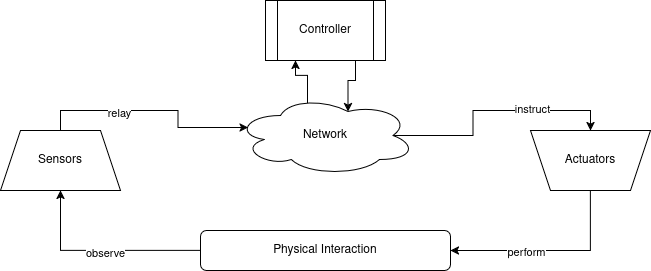
\includegraphics[width=0.7\textwidth]{graphics/cpsGeneralArchitecture.png}
  \caption{General architecture of common CPS}
  \label{fig:cps_architecture}
\end{figure}


Controllers may range from simple reactive routines to advanced inference models grounded in probabilistic programming, or even intelligent agents capable of autonomous
decision-making. Actuators, in turn, translating these decisions into physical action can be represented by basic devices such as motors that move parts,
valves that regulate flow, or relays that control circuits. They can also act as more complex assemblies - robotic joints, programmable hydraulic systems, or smart actuators
that adjust based on local conditions. At the foundation, sensors continuously monitor the environment, capturing data through modalities such as motion,
orientation, or spatial mapping. Together, these elements form  an integrated feedback system, enabling CPS to respond intelligently and flexibly to their physical context,
regardless of application domain.\\

CP-Systems are inherently multidisciplinary structures intersecting engineering domains (mechanical, electrical, civil, etc.) with computer science.
Because these domains employ differing models for ... , effectively combining them is non-trivial. Challenges arise during development and operation of CPSs for which
finding solutions is imperative. \cite{cpsChallengesAndFuture} First and foremost is the concern of \textbf{reliability and safety}. Occurrences of failures can have dire real-world
consequences with catastrophic end results. This means systems must handle unexpected conditions gracefully and robustly. But ensuring safety through extensive verification
and validation is complicated by the combination of continuous physical dynamics and discrete decision logics. Another challenge is \textbf{real-time performance}, as computing
elements must keep pace with the physical processes, which usually require low-latency responsiveness including the network. Since CPSs are used in infrastructure and other
critical sites that may be targets of cyber attacks, guarantying a high standard of \textbf{Security} is essential. Additionally, sensors are not completely reliable -
possibly introducing noise to measurements - and environmental conditions can vary drastically leading to \textbf{uncertainty}, which a CPS has to cope with to be resilient. \cite{cpsProbabilisticRobotics}

\label{sec:formal-methods}
\section{Formal Methods and Model Checking}

CPSs are often deployed in safety-critical environments where utmost importance is placed on reliable operation and functional correctness. Yet reaching high levels of confidence
in a systems behavior remains extremely inside cyber-physical domains.\cite{formalMethodsCPSCritical} This difficulty arises from the complex interactions of all the individual integral
components of the system, which can not be effectively tested only employing traditional methods. The inherent entanglement of these systems warrants the use of
specialized procedures that are able to cover and validate the acting components. Unlike conventional simulation based testing, \textit{formal methods} are able to prove correctness against
formal specifications, thereby providing more reliable results and eliminating potential error sources, such as race conditions or violations of safety properties(unnoticed states).

In formal methods, \textit{theorem proving}, \textit{model checking}, and \textit{runtime verification} are widely recognized as the three main approaches for assuring
system correctness\cite{formalMethodsBig3,formalMethodsCPSCritical}.
All three practices are distinguishable from one another and are tailored for certain scenarios. Runtime verification is a lightweight technique that verifies systems
by inspecting their execution trace - often employing automata to detect violations. Theorem proving, in contrast, is an offline and often time intensive
process relying on mathematical inference rules to statically validate correctness with a high degree of rigor.\\

Model checking is of most interest in this case, as the MiniProb DSL \ref{sec:miniprob} was developed with this context in mind. \cite{POPACheck}
It statically verifies a system by exhaustively exploring the state-space and is considered one of the most successful verification techniques. \cite{formalMethodsCPSCritical}
The thorough analysis of reachable states, combined with specifications which are expressible in various forms of modal logic,
offer a strong expressive foundation for property verification \cite{modelCheckingPrinceples}. However, the systematic exploration of states leads to poor performance, especially for model with
complex and big state spaces. Moreover, as most model checking implementation employ automata-based solutions, systems are usually converted into
equivalent state machines which can result in an explosion of states.\cite{}
Model checking is generally only used in conjunction with finite-state machines for aforementioned reasons. Still, theres been advances trying to apply it to infinite state spaces.
\cite{modelCheckingInfCounter,modelCheckingInfSymb}. The resulting verdicts for infinite-state models are typically approximations or are restricted by bounded analysis,
such as checking only a finite number of steps or abstracting unbounded data domains. As a result, the verification outcomes may not provide absolute guarantees for all
possible executions, but rather assurances that hold under specific assumptions, abstractions, or within predefined limits of a system's behavior.

These approaches often rely on \textit{symbolic evaluation} rather than naive enumeration of states. By representing potentially infinite sets of states using logical
formulas or data structures such as Binary Decision Diagrams (BDDs) or SMT formulas, symbolic model checking can reason about system behavior without explicitly
generating every state.

\section{Motivation for PPLs in CPS Contexts}

Probabilistic programming has multiple fitting applications within CPSs, especially where reasoning under uncertainty is essential. Generally, probabilistic programming
allows controllers to plan even in unpredictable environments and settings.

\begin{multicols}{2}
  \begin{itemize}
    \item When measurements contain noise or are incorrect, PPL models can still be applied to extract useful information. Instead of treating the raw reading of a sensor as the “truth,”
  the readings are considered samples for a \textit{sensor’s model}. Not only is it possible to reduce the noise in the measurements by calculating the posterior,
  but those noise characteristics are also used to flesh out the predictive model itself.
  This enables PPLs to adaptively adjust noise models online when, for example, sensors deteriorate over time.
  Additionally - with most CPSs employing multiple sensors - a PPL naturally supports \textit{sensor fusion}, \cite{cpsSensorFusion} combining data from heterogeneous sources
  to produce a coherent estimate. By defining each sensor's observation as a conditional distribution, a probabilistic program
  weights each reading according to its uncertainty: more reliable sensors contribute more heavily, while inconsistent or faulty readings are down-weighted or flagged.
  Inference then yields a joint posterior over the true state, allowing the system to reconcile disagreements between sensors, detect potential sensor failures by inferring
  latent bias variables, and maintain a quantified confidence.
  \item Which leads us into robotics, a quintessential cornerstone of CPS. Instead of working on raw observational data and making assumptions in incomplete cases, robots can adopt
  a \textit{belief} based on an observational model \cite{cpsProbabilisticRobotics}. The observational model couples motion dynamics (how actions translate into state
  transitions) with existing sensor models, providing a full posterior distribution that the robot can use to imply different levels of confidence for its actions.
  Furthermore, robots often operate in changing environments or with components that degrade over time. Within a PPL, unknown parameters, such as friction
  coefficients or sensor calibration offsets, can be treated as latent variables and perform Bayesian learning to infer them from incoming data. The same inference mechanism used for state
  estimation thus also adapts the model online, continuously refining both motion dynamics and sensor mappings.
  
  \item A PPL expresses system dynamics probabilistically so that sampling yields a distribution of possible futures. \cite{cpsPredictiveControl} By enforcing “chance constraints”
  (e.g., “limit the probability of exceeding a safety threshold to 1\%”), inference or Monte Carlo sampling identifies control inputs that optimize expected performance while
  respecting risk. When the current state is uncertain, planning occurs in belief space - each action triggers a Bayesian update of the state distribution, and planners
  choose sequences that minimize expected cost given that uncertainty. Simultaneously, online Bayesian learning refines model parameters (like friction or drag) over time,
  tightening future predictions; as uncertainty shrinks, control can push closer to limits, whereas rising uncertainty leads to more conservative actions.
  
  \item Recent research is looking at ways to utilize PPLs to gather diagnostics of a CPS. \cite{cpsPPLDiagnostics} They authors propose a way to infer potential error causes, that
  might be overlooked otherwise, due to the .
  This of of great interest to system operators for deciding if either parts have to be replaced or only have to be recelebrated. Because measured data on system deviations
  often reflects complex intertwining causes and \textit{closed-loop corrections}, identifying root causes becomes a matter of inference. The proposed two-step approach
  first builds a generative model (based on control software and expert insights) that simulates observations from hypothesized error causes. This simulator is then recast
  as a probabilistic program, allowing Bayesian inference to estimate latent causes (with confidence intervals) from actual measurements.

  \end{itemize}
\end{multicols}

\label{sec:pp}
\chapter{Probabilistic Programming}
\section{What Is Probabilistic Programming?}

Probabilistic programming is a paradigm that aims to perform statistical analysis using tools yielded by computer science.\cite{introductionprobabilisticprogramming}
Unifying general-purpose programming and probabilistic modelling enables the presentation of statistical models as a program. Defined by underlying program code, the model is
embodied by the relations between variables and calculations. The established capabilities of programming languages are often augmented with
probabilistic functionality, in ... creating probabilistic programming languages (PPL),\cite{probProgrammingPrinciples,2025modelcheckingprobabilisticoperator}
that are closely associated with this paradigm.
The enriched syntax enables the creation of more compact models and fosters conciser abstractions of the underlying probabilistic structure, usually providing constructs
that allow declaring random variables and conditioning of observed data. These primitives form the foundation for specifying core elements
of statistical models. \textit{Priors} are pre-known and usually drawn from distributions reflecting the initial belief over what value
\textit{latent variables}/model parameters might take on. \textit{Likelihoods} are also known beforehand representing how data is assumed to be generated given the
latent variable for which the \textit{posterior} is to be inferred. Together, these components form the backbone of a probabilistic model and provide the information required
to compute the posterior distribution, which is grounded in \textbf{Bayesian theory}.\cite{introductionprobabilisticprogramming}
\\

\textit{Bayes’ Theorem} provides the foundational framework for probabilistic reasoning under uncertainty. It describes how to update prior beliefs about unknown
quantities - known as latent variables - based on new evidence, resulting in a posterior distribution. Formally, it states that the posterior is proportional to the
product of the prior and the likelihood:
\[
  P(\theta \mid x) \propto P(x \mid \theta) \cdot P(\theta)
\]
In probabilistic programming, this principle is applied through models that define prior distributions over latent variables and likelihood functions for
observed data. The probabilistic programming language then applies Bayes' Theorem, typically via automated inference algorithms, to compute or approximate the posterior.
This makes it possible to express complex probabilistic models declaratively, while delegating the computation of posterior beliefs to the underlying inference engine.
\\

\section{Inference and Sampling Methods}

Inference is the process by which probabilistic models are "executed". Given a model and observed data, the task is to compute the posterior distributions of latent variables.
Because probabilistic models often include uncertainty and hidden variables, inference is the process that turns the model into concrete answers.
This process is abstracted and automated, but remains computationally nontrivial. Standard approaches to inference are generally grouped
into three main categories- \textit{exact inference}, \textit{sampling-based methods}, and \textit{variational inference}.\cite{bishop2006prml, blei2017vi, goodman2014dippl}.

\subsection*{1. Exact Inference}

Exact inference computes the posterior distribution analytically or through complete enumeration. This is possible only in models with limited complexity where the
entire state space can be traversed. Although conceptually straightforward, exact inference quickly becomes infeasible as model size increases, due to the combinatorial
explosion of possible states.

\subsection*{2. Sampling-Based Inference}

Sampling-based inference approximates the posterior by drawing samples from it, typically using Markov Chain Monte Carlo (MCMC) methods.
Continuously, random samples are generated from a given distribution - usually the prior or a conditional- and used to progressively approximate
the posterior with the model being executed repeatedly.
These approaches are flexible and can handle complex models, but they are often computationally expensive and require many samples to ensure accuracy.
The resulting samples can then be used to estimate expectations, marginal distributions, or event probabilities.

\subsection*{3. Variational Inference}

Variational inference formulates inference as an optimization problem. Instead of sampling, it produces a family of approximate distributions and seeks the member that
is closest to the true posterior. This involves defining an objective function - often the \textit{evidence lower bound (ELBO)} - and optimizing it using gradient-based methods.
Variational inference tends to be faster and more scalable than sampling, though it trades off exactness for speed by approximating the posterior rather than sampling
from it directly \cite{blei2017vi}.


\begin{figure}[htbp]
  \centering
  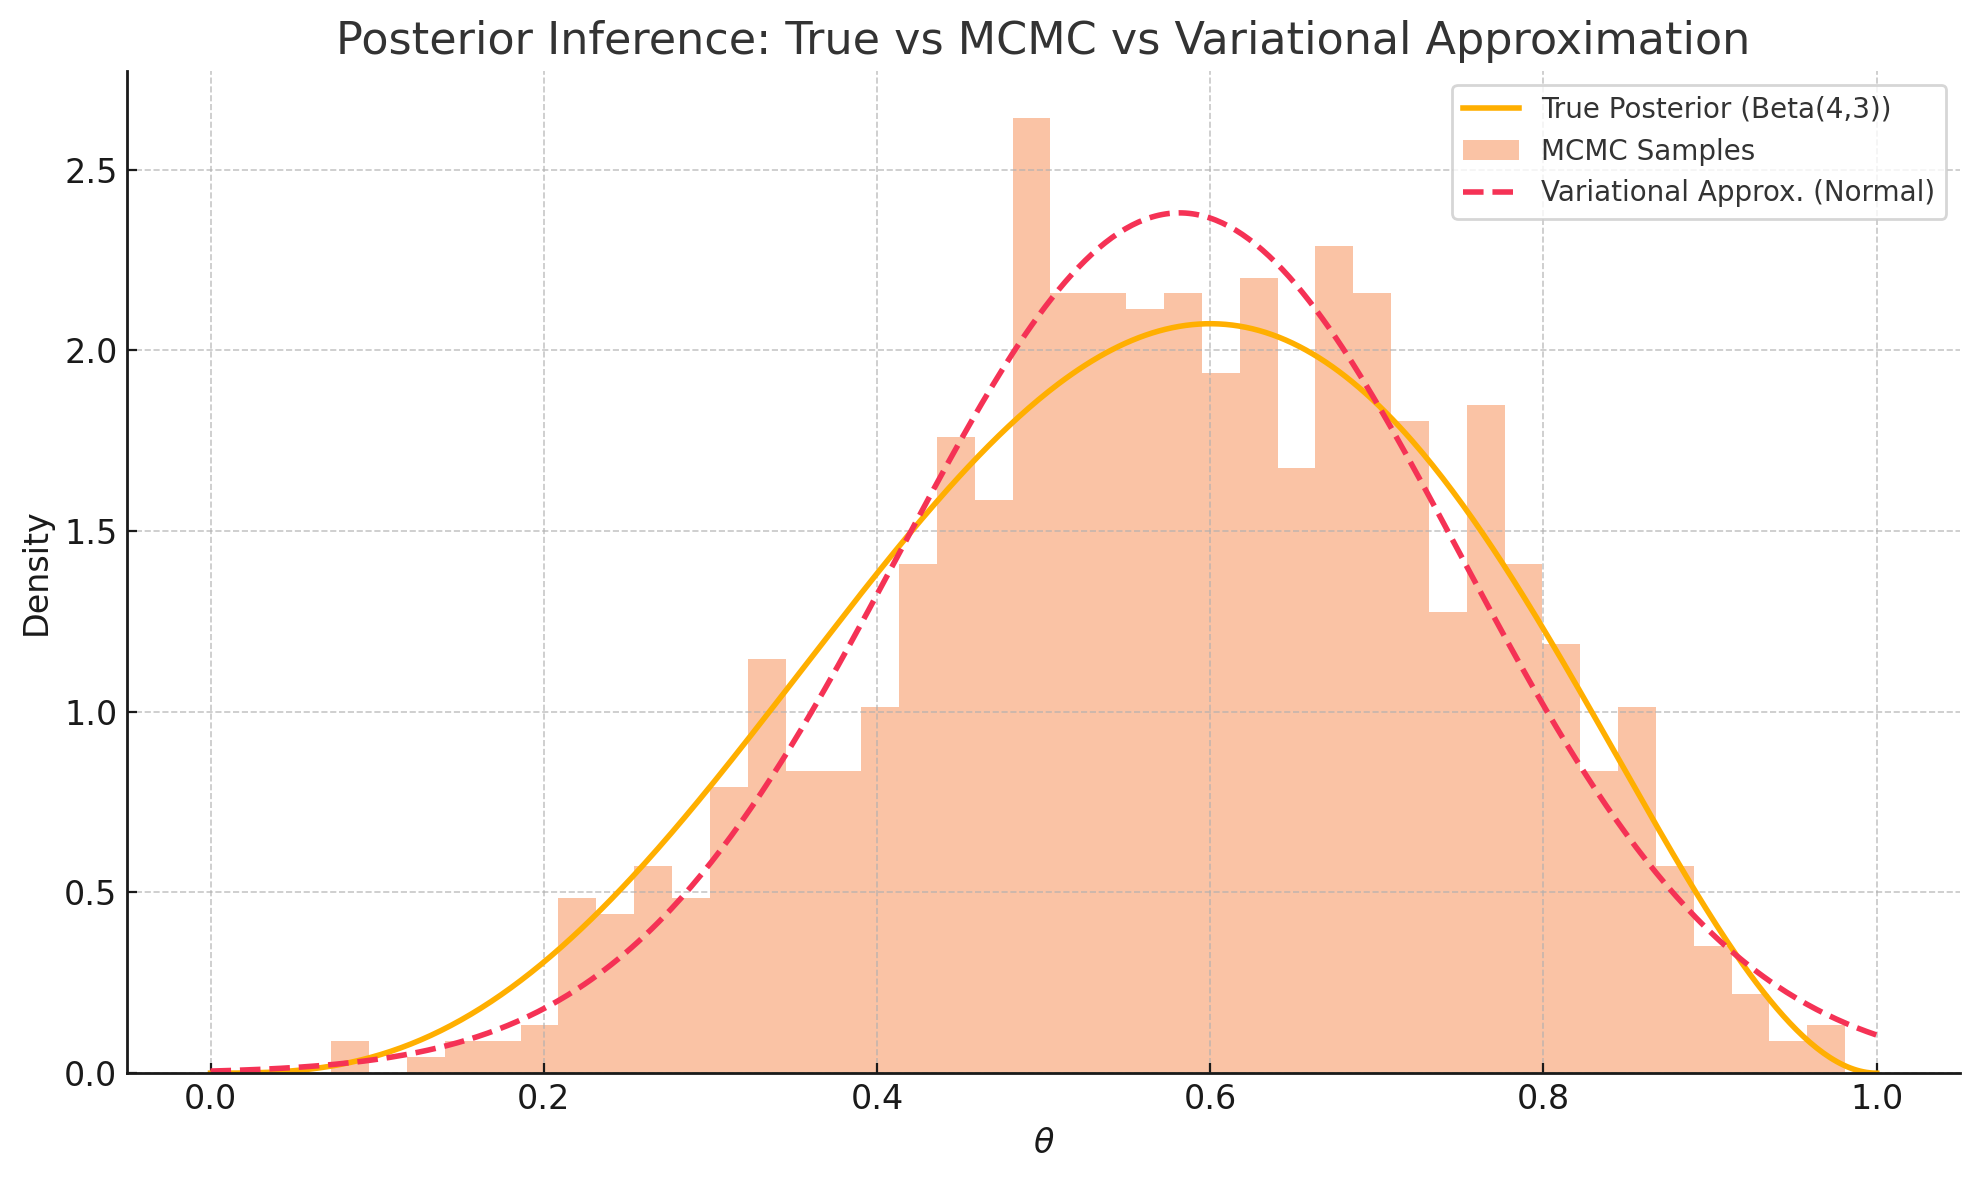
\includegraphics[width=0.7\textwidth]{graphics/inferencePlot.png}
  \caption{Comparison sample of exact posterior to inference methods}
  \label{fig:inference_plot}
\end{figure}

\section{Symbolic Semantics and Model Checking}

While probabilistic programming is typically associated with statistical inference and sampling-based evaluation, there exists an alternative perspective
that treats probabilistic programs as formal models subject to verification \cite{2025modelcheckingprobabilisticoperator,sato2019formal} as described in \ref{sec:formal-methods}.
In contrast to traditional inference, symbolic evaluation and model checking aim to rigorously analyze all possible executions of a program against formal specifications.

Symbolic approaches differ in that they do not enumerate individual executions or samples, but instead reason over entire sets of possible states and paths using
abstract representations. This enables analysis of program behavior in a more in-depth and automated way, making it possible to answer questions like:
“Does this property always hold, regardless of sampling outcomes?” or “What is the probability that this condition is eventually satisfied?”

Such techniques are particularly relevant for verifying probabilistic systems where correctness, safety, or reachability must be guaranteed rather than estimated.
They also enable reasoning about programs that would be challenging to analyze through sampling alone, such as those involving recursion, nondeterminism, or infinite state
spaces.

A growing body of foundational work has explored how symbolic and model checking techniques can be adapted to probabilistic
settings \cite{BaierClarkeHartonasGarmhausenKwiatkowskaRyan1997,EsparzaKuceraMayr2006,EtessamiYannakakis2012}. This includes approaches based on probabilistic automata, logics for probabilistic reasoning, and
symbolic representations of state spaces.

Building upon these foundations, the POPACheck tool \cite{POPACheck} represents a pioneering approach to verifying probabilistic programs with recursive structure.
By translating programs into probabilistic operator precedence automata - a formal model that can represent infinite state spaces - POPACheck allows for the analysis
of properties expressed in structured temporal logics. This enables verification of systems that lie beyond the scope of most traditional probabilistic programming
frameworks.

In this context, \emph{MiniProb} is used not for inference, but as a front-end language for describing probabilistic behavior that is ultimately verified through
model checking. The distinction between sampling-based execution and symbolic verification is presented below.

\section{Methodological Comparison}
\begin{table}[h]
  \centering
  \caption{Comparison of Probabilistic Programming in Traditional Inference vs. Formal Verification}
  \begin{tabular}{|p{4.5cm}|p{5.5cm}|p{5.5cm}|}
    \hline
    \textbf{Aspect}           & \textbf{Traditional Inference (e.g., Bayesian Modeling)}                      & \textbf{Formal Verification (e.g., Model Checking)}                                    \\
    \hline
    Primary Goal              & Estimate posterior distributions over variables (e.g., $P(\theta \mid data)$) & Prove correctness properties about probabilistic behavior (e.g., reachability, safety) \\
    \hline
    Evaluation Strategy       & Sampling-based execution (e.g., MCMC, SMC, VI)                                & Symbolic or exhaustive exploration of probabilistic state space                        \\
    \hline
    Execution Semantics       & Program runs as a simulator; samples are drawn during execution               & Program is interpreted mathematically; all behaviors are analyzed systematically       \\
    \hline
    Handling of Randomness    & Uses actual draws from distributions during execution                         & Treats random variables symbolically or via full enumeration                           \\
    \hline
    Output                    & Posterior samples, estimates, and confidence intervals                        & Probabilistic bounds, expected values, or formally verified properties                 \\
    \hline
    Typical Model Assumptions & Often uses continuous distributions and models real-world noise               & Often restricted to discrete, well-defined models for tractability                     \\
    \hline
    Result Guarantees         & Approximate; dependent on convergence and diagnostics                         & Sound (and often complete) within model and logic constraints                          \\
    \hline
  \end{tabular}
  \label{tab:inference_vs_verification}
\end{table}


\label{sec:miniprob}
\chapter{The \textit{MiniProb} DSL}
\section{Domain and Purpose}
\textit{MiniProb} is the successor of a DSL first introduced as \textit{MiniProc}\cite{miniproc}. Originally lacking the typical probabilistic
primitives such as \code{observe} and \code{query}, the language was designed for formal verification of recursive programs (see: \ref{sec:formal-methods}). As MiniProc focuses on recursive control-flow and
call-return semantics - qualities representative of procedural programming - it classifies under the imperative paradigm (see \ref{sec:prog-paradigms}). Furthermore, it is a
context-free language, since its structure is tightly coupled with the theory of \textbf{Operator Precedence Languages (OPLs)}, a deterministic subclass of CFLs (see: \ref{sec:formallangs}).
Programs written in MiniProc can be directly compiled into \textbf{Operator Precedence Automata (OPA)}, which leverage the structured nesting of procedure calls and
returns, thus enabling automata-based model checking via the \textit{POMC} tool against specifications written in the Precedence-Oriented Temporal Logic (POTL) \cite{miniproc}.
This conversions is made possible because MiniProc constraints its syntax to comply with the \textit{precedence relations} defined by a given
\textbf{Operator Precedence Matrix (OPM)}, allowing for deterministic and unambiguous parsing.
??MAKE SHORTER (note) same for PTLfx below??
\marginpar{}
\\

MiniProb extends MiniProc by incorporating primitives from PPLs \cite{POPACheck}, which enable sampling, conditioning and nested inference (see: \ref{sec:pp}).
While remaining recursive-procedural, it now belonging to the family of probabilistic programming languages, still within the context-free class, but no longer parsable to an OPA.
However, with the introduction of non-determinism and probabilistic transitions, MiniProb programs are able to be translated into
\textbf{probabilistic Operator Precedence  Automata (pOPA)} \cite{POPACheck,2025modelcheckingprobabilisticoperator}, that can represent both stack and stochastic behavior.
This transition enables formal verification of MiniProb programs via model checking, supporting \emph{qualitative}, \emph{quantitative}, and \emph{approximate} queries,
allowing to check whether properties - specified in $POTLf_\chi$ - hold with certainty, compute exact satisfaction probabilities, or obtain estimated bounds when exact computation is infeasible \cite{guideMiniProb}.

\begin{quote}
  POTL is a temporal logic specifically designed to express properties over Operator Precedence Languages (OPLs) \cite{chiari2020potlfirstordercompletetemporal,Chiari_2022}.
  Extending LTL, it includes modalities that refer to the hierarchical structure induced by procedure calls and returns,
  enabling formal reasoning about context-sensitive behaviors such as matching call-return sequences, stack inspection, and structured exception handling.
  The fragment POTL\textsubscript{$f_\chi$} restricts the logic to a form suitable for model checking over non-deterministic and probabilistic systems - particularly when
  used with probabilistic Operator Precedence Automata (pOPAs) - while retaining the expressive power needed to reason about structured control flows \cite{2025modelcheckingprobabilisticoperator}.
\end{quote}

MiniProb also incorporates expressing higher-order reasoning patterns, such as those involving mutually recursive queries that simulate agents reasoning about each other's
beliefs or decisions - a feature common in cognitive modeling and multi-agent systems \cite{multiAgent}.

As a DSL, MiniProb is not intended to offer the general-purpose capabilities of mainstream languages. In particular, it is not Turing-complete:
it lacks features like unbounded memory manipulation, arbitrary recursion without termination guarantees, or dynamic data structures. Its constructs are deliberately
limited to ensure compatibility with pOPA translation and to preserve decidability of model checking, which would not be possible in a fully general computational model.
\\

Ultimately, the purpose behind both MiniProc and MiniProb is to offer a high-level, user-friendly interface for programmers wishing to verify properties of recursive (probabilistic) programs without needing to manually translate their source code into OPA or pOPA representations. These DSLs thus serve as a crucial bridge between real-world programming constructs and the formal models required for rigorous verification.

\section{Syntax}

\begin{wrapfigure}{l}{0.5\textwidth}
  \centering
  \[
    \begin{array}{rcl}
      prog
       & \to  & (decl\;\texttt{;})^* \;func^+                                                     \\[6pt]

      decl
       & \to  & type\;\mathit{id}\;(\texttt{,}\;\mathit{id})^*                                    \\[6pt]

      func
       & \to  & \mathit{id} \texttt{(}
      (\,type\;\texttt{\&}?\;\mathit{id}
      (\texttt{,}\;type\;\texttt{\&}?\;\mathit{id})^*\,)?
      \texttt{)}                                                                                  \\[-2pt]
       &      & \texttt{\{}(decl\;\texttt{;})^*\;stmt^+\texttt{\}}                                \\[6pt]

      fcall
       & \to  & \mathit{id}\;\texttt{(}
      [\,e\;(\texttt{,}\;e)^*\,]
      \texttt{)}                                                                                  \\[6pt]

      stmt
       & \to  & lval\;\texttt{=}\;e\;\texttt{;}                                                   \\[-2pt]
       & \mid & lval\;\texttt{=}\;\texttt{Distribution(...)}\;\texttt{;}                          \\[-2pt]
       & \mid & (\texttt{query})?\;fcall\;\texttt{;}                                              \\[-2pt]
       & \mid & \texttt{observe}\;e\;\texttt{;}                                                   \\[-2pt]
       & \mid & \texttt{throw}\;\texttt{;}                                                        \\[-2pt]
       & \mid & \texttt{if}\;\texttt{(}e\texttt{)}\;\{\;stmt^*\;\}\;\texttt{else}\;\{\;stmt^*\;\} \\[-2pt]
       & \mid & \texttt{while}\;\texttt{(}e\texttt{)}\;\{\;stmt^*\;\}                             \\[-2pt]
       & \mid & \texttt{try}\;\{\;stmt^*\;\}\;\texttt{catch}\;\{\;stmt^*\;\}                      \\[6pt]

      lval
       & \to  & \mathit{id}\;(\texttt{[}e\texttt{]})?                                             \\[6pt]

      type
       & \to  & \texttt{bool}
      \;\mid\;(s\mid u)\;int\;(\texttt{[}int\texttt{]})?                                          \\[6pt]
    \end{array}
  \]
  \caption{Compacted grammar of \texttt{MiniProb}.}
  \label{fig:ebnf_grammar}
\end{wrapfigure}

??reference to BNF of MiniPRob from BNF section??

A compacted grammar for MiniProb is shown in \ref{fig:ebnf_grammar} containing the core elements for intuitive comprehension.
A full BNF grammar can be found in the appendix see \ref{fig:bnf_grammar}.
A \emph{prog} consists of zero or more top-level declarations followed by one or more function definitions. Each \emph{decl} introduces one or more variables of a
given \emph{type}, which may be \code{bool}, signed (\code{s}) or unsigned (\code{u}) integers of certain bit-width (e.g., \code{s8}, \code{u16}),
and optionally fixed-size arrays (e.g., \code{u8[10u4]}). Functions (\emph{func}) consist of an identifier, an optional list of typed parameters (passed by value or
reference via \code{\&}), and a block containing optional local declarations and at least one statement.

Within function bodies, MiniProb allows for local declarations and familiar C-like statements, including variable assignments (\code{lval = \emph{e};}),
function calls, and control flow structures such as \code{if}/\code{else}, \code{while} loops, and structured exception handling via \code{try}/\code{catch},
with \code{throw;} used to abort execution. Left-hand values (\emph{lval}) may refer to scalar variables or indexed array elements, while types follow a compact
convention, consisting of Booleans and signed or unsigned integers of fixed width.

Probabilistic constructs are central to MiniProb's design. These include sampling from distributions via statements like \code{lval = Distribution(...);},
currently supporting both \code{Bernoulli} and \code{Uniform} distributions. The \code{observe \emph{e};} construct allows conditioning execution on logical expressions,
rejecting traces that do not satisfy the observed condition. Inference is triggered through the \code{query \emph{fcall};} statement, which indicates
the probability evaluation of a function's outcome given a set of observations.

In addition to structured control, MiniProb supports expressions built from literals, variables, and function calls, composed using arithmetic
operations (\code{+}, \code{-}, \code{*}, \code{/}, \code{\%}), comparison operators (\code{==}, \code{!=}, \code{<}, \code{<=}, etc.), and Boolean connectives
(\code{!}, \code{\&\&}, \code{||}). These expressions can appear on the right-hand side of assignments or as arguments.

Beyond the standards, MiniProb introduces \emph{probabilistic assignments} to express uncertain choices: $lval = e_1 \{ e_2 : e_3 \} \; e_4$.
This construct selects $e_1$ with probability $p = e_2 / e_3$, and $e_4$ with probability $1 - p$.
Multiple such choice blocks can be chained to define multi-way probabilistic decisions, enabling a compact encoding of stochastic control.

Identifiers follow the pattern \code{[a-zA-Z\_][a-zA-Z0-9.\_\:$\sim$]*}, allowing names with symbols like underscores, colons, dots, and tildes.
Integer literals are annotated explicitly with both value and type, e.g., \code{42s8}, \code{7u16}, where the suffix denotes signedness and bit width.
Boolean literals are written plainly as \code{true} and \code{false}.
\\

Lastly, MiniProb also includes a few more constructs which are omitted here as, they are currently not covered by the language extension.
These constructs include \code{probabilistic query: ...} defining the type of query, \code{formulas = ...}: specified by POTL formalisms and the definition of \emph{modules} \cite{guideMiniProb}.

\section{Semantics and Example Models}

To support reliable analysis and ensure well-formed behavior, MiniProb enforces a few core semantic rules. Each program must include a \texttt{main} function with no parameters. When passing arguments by reference (value-result), the actual argument must be a variable identifier rather than a literal or expression. Additionally, the \texttt{query} construct can only be used on functions that declare at least one reference parameter.

These rules are exemplified in the following implementation of a simplified \textit{Schelling coordination model}. In this setup, two agents - Alice and Bob - independently choose between two cafés, preferring to coordinate without direct communication. Each agent samples an initial preference, then recursively queries the other's decision to adjust its own. The model uses probabilistic sampling and mutual \texttt{query} calls, while \texttt{observe} enforces alignment between the agents’ choices. The shared variable \texttt{p} bounds recursion depth, ensuring termination.
\begin{figure}[ht]
  \centering
  \begin{minipage}{0.85\textwidth}
    \begin{minted}[fontsize=\small]{c}
program:
u4 p;
main() {
  bool res;
  p = 11u4;
  query alice(res);
  // res is which café they have gone to
}

alice(bool &x) {
    bool prior_alice, bob_choice;
    // sample according to the prior (0.55)
    prior_alice = 1u1 {11u5 : 20u5} 0u1;
    p = p - 1u4;
    query bob(bob_choice);
    observe prior_alice == bob_choice;
    x = prior_alice;
}

bob(bool &y) {
    bool prior_bob, alice_choice;
    // sample according to the prior (0.55)
    prior_bob = 1u1 {11u5 : 20u5} 0u1;
    if (p > 0u4) {
        query alice(alice_choice);
        observe prior_bob == alice_choice;
    } else {}
    y = prior_bob;
}
\end{minted}
  \end{minipage}
  \caption{MiniProb implementation of the Schelling coordination model.}
  \label{fig:schelling}
\end{figure}
\end{refsection}

%=== Part II - Design & Implementation ===%
\begin{refsection}
  \part{Design \& Implementation}
  \chapter{Requirements and Technological Context}

As discussed in in the introduction \ref{sec:scope}, the main aim is the development of a VS Code Language extension that operates on par with
well-established tooling for other programming languages. The following requirements define the expected capabilities and characteristics the extension must demonstrate.

\begin{multicols}{2}
  \subsection*{Functional Requirements}
  \begin{enumerate}
    \item The extension must provide syntax highlighting for the target language, differentiating keywords, operators, literals, and identifiers.
    \item The extension must provide basic code completion suggestions based on language keywords and the abstract syntax tree (AST) generated by Langium.
    \item The extension must be able to validate data types within the language, providing warnings or errors when type mismatches occur.
    \item The extension must perform semantic analyses to detect invalid constructs, undefined variables, and other semantic errors.
    \item The extension must display syntax and semantic error messages in the editor in real-time as the user edits the code.
    \item The extension must utilize the Langium framework for language specification, parser generation, and language service implementation.
  \end{enumerate}

  \columnbreak

  \subsection*{Non-Functional Requirements}
  \begin{enumerate}
    \item The extension must respond to user edits with syntax and semantic feedback within 100-250ms for files of average size.
    \item The extension must provide a user-friendly experience that is consistent with other popular VS Code extensions.
    \item The extension must be structured and commented in a way that allows future developers to understand and extend its functionality easily.
    \item The extension must be compatible with the latest version of Visual Studio Code at the time of its release and be developed using Langium, with consideration for future maintenance and version support.
    \item The extension must be able to handle files of immense size (around 10000 lines) of code within the bounds of 1 second.
    \item The extension must be delivered with clear and comprehensive documentation, including installation, usage, and extension of its features.
  \end{enumerate}
\end{multicols}

\section{Alternative Technologies}

This extension is implemented using \textbf{Langium}, which itself builds upon the standardized \textbf{Language Server Protocol (LSP)} \cite{LSP}, yet
there are several other technologies and approaches available for creating Visual Studio Code language extensions. At its core, the LSP allows tooling for programming
languages to be developed in a modular, editor-independent manner, making it possible to implement a language server in any language that can communicate via JSON-RPC.

One common approach is to implement a language server using general-purpose programming languages (e.g., TypeScript, Java, or Rust) combined with parser generation libraries.
Technologies such as \textbf{Jison}~\cite{Jison}, \textbf{Nearley}~\cite{Nearley}, and \textbf{PEG.js}~\cite{PEGjs} offer a range of options for specifying a language's grammar
and creating a parser. These libraries vary in design and capabilities and may need extra components, such as dedicated lexers and scoping to enable fully-fletched tooling.

In contrast, more comprehensive technologies such as \textbf{ANTLR}~\cite{ANTLR} and \textbf{Langium} go beyond
basic parsing. ANTLR provides a mature and highly optimized lexer and parser generation framework that is widely used across many programming languages, while Langium offers
an end-to-end solution for language engineering - including built-in support for scoping, indexing, and validation - making it especially suited for creating fully
featured language servers.

For basic syntax highlighting and lexical analysis, \textbf{TextMate}-style grammars~\cite{TextMate} can be used, offering a lightweight approach when deep semantic understanding is not required.
Meanwhile, incremental parsing frameworks such as \textbf{Tree-sitter}~\cite{Treesitter} have gained popularity for their ability to provide high-performance syntax parsing and error recovery,
making them ideal for tooling that operates on very large files.

\chapter{Langium}

Langium is a young language engineering framework inspired by the accomplishments of \verb|Xtext|, striving to evolve into a similarly comprehensive and widely-used technology stack.\cite{LangiumWeb}
Its goal is to lower the barrier to entry for language design and implementation, opening the field to new users and fostering the growth of its user base.
To achieve this, Langium embraces the extensibility of the Visual Studio Code ecosystem and its extension pipeline, provides a rich set of built-in
capabilities while strongly focusing on quality and maintainability, ensuring that newcomers and experienced developers alike can build robust, sustainable language tooling.

Although Langium is capable of defining general-purpose languages, its design is primarily optimized for domain-specific languages (DSLs), targeting languages with a limited range of abstraction and complexity.
Creating a fully featured GPL is a highly exhaustive endeavor that demands extensive semantic modeling, thorough tooling, and a substantial team of developers.
In contrast, Langium is tailored to lower the entry barrier for language design, making it an ideal choice for building DSLs that solve specific, well-defined problems.
\\

\section*{Technical Details \& Features}

Langium is an open-source framework for building programming languages and DSL tooling, distributed under the MIT license and backed by the Eclipse Foundation \cite{LangiumGit}.
Its open-source nature encourages collaboration and continuous improvement through active engagement with the community.
\begin{multicols}{2}
  \begin{itemize}
    \item At its core, Langium builds upon \verb|Chevrotain|, a customizable JavaScript parser engine that is highly optimized. Chevrotain constructs an internal prediction DFA \cite{sujew2022enabling}
          from the grammar's production rules to implement its configurable LL($k$) lookahead mechanism, allowing the look-ahead depth $k$ to be tuned for both performance and
          expressiveness. Moreover, Langium exposes this configurability directly - authors can adjust the parser's \verb|maxLookahead| setting to manage grammar complexity and
          parsing speed. After parsing, Chevrotain produces a Concrete Syntax Tree (CST), which Langium then converts into a typed Abstract Syntax Tree (AST) using the visitor pattern:
          by extending Chevrotain's own Visitor interface, Langium traverses the CST and emits AST nodes, preserving semantic structure while discarding syntactic noise.
          Langium does not incrementally parse documents (i.e., it does not reuse prior parse results to update only modified regions), yet it still offers significant performance
          benefits compared to alternative engines \cite{Chevrotain}, complementing its generation of precise ASTs and CSTs and its robust error recovery capabilities. The error recovery is
          implemented with single-token insertion and deletion strategies to correct unexpected or missing tokens, alongside rule-level resynchronization that discards input until a defined
          recovery point is reached, to maintain parser continuity in the face of syntax errors.
    \item Langium provides a custom DSL using the \code{.langium} extension to define the grammar on which everything else is built upon. This DSL closely resembles an EBNF grammar,
          augmenting basic BNF with regex-like operators, language constructs for assignments and typing, and built-in cross-referencing. Cross-referencing enables production rules to declare relations to one another, which are resolved during a document's linking phase.
          Once defined, the core grammar is converted into a Chevrotain compatible JSON view, which when consumed by the parser, produces a fully typed AST. While linking, the AST is traversed and any
          cross-references resolved by checking the reference against the computed scope of each possible reference holder.
    \item In addition to its core language capabilities, Langium offers further extensibility: its generator API traverses ASTs and CSTs to produce arbitrary outputs
          - whether transpiled or compiled code, structured data formats such as JSON, XML, or Markdown, or custom domain-specific representations - and thus supports downstream
          processing, tooling, or integration into build and deployment pipelines.
          Langium projects can also be scaffolded into a command-line interface, registering commands for parsing, validation, generation, and LSP serving; each command invokes the
          corresponding language services to parse source files, apply validation rules, execute generator or interpreter routines, and emit results, thereby enabling a cohesive
          suite of tools, that leverage Langium's core capabilities across diverse environments.
    \item Leveraging established and widely adopted ecosystems is central to the design of Langium, allowing it to benefit from mature tools, protocols, and conventions.
          As a result, it adopts the LSP - standardizing language tooling across platforms and environments - to enable seamless integration with editors and IDEs such as Visual Studio Code and Eclipse Theia.
          In the same vein, it is developed in TypeScript and distributed via npm, which allows it to build upon the robust tooling, typing support, and package infrastructure of the JavaScript and TypeScript landscapes.
    \item To further streamline the DSL development process, Langium provides a dedicated scaffolding tool based on \verb|Yeoman|. This generator automates the creation of a
          fully configured project, including a grammar template, build pipelines, and example code for parsers, validations, and editors. Removing boilerplate setup provides a
          standardized structure to build upon and saves developers significant time and effort, making Langium a practical and accessible platform.
  \end{itemize}
\end{multicols}

\section{High-Level Architecture Diagram \& Module Decomposition}
\begin{figure}
  \centering
  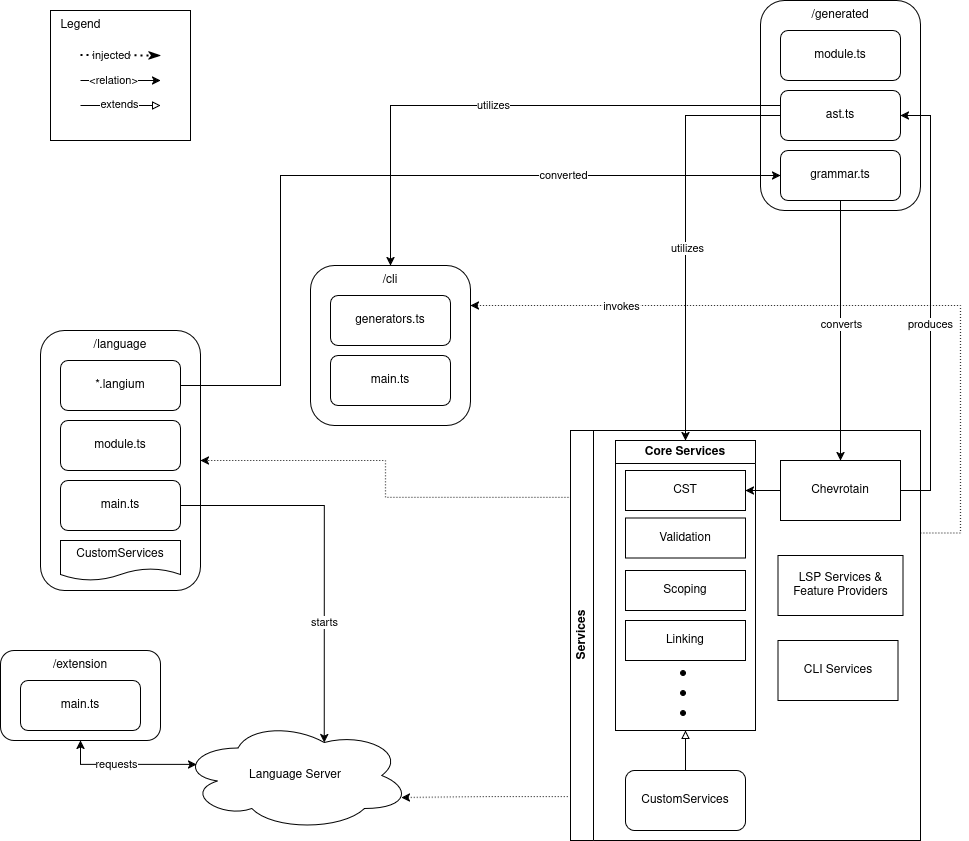
\includegraphics[width=\textwidth]{graphics/langiumArchitecture.png}
  \caption{Architecture overview of a Langium project}
  \label{fig:langium-architecture}
\end{figure}

Langium projects can easily be created with the support of the scaffolding tool \verb|Yeoman|, producing a structured mock project including a sample language definition.
Most of the definitions are found in the \verb|src| directory \ref{fig:langium-architecture}, encompassing functionality for the Language Server, the extension and actual language tooling.

\begin{description}
  \item[\code{language/}] Assembles the core of any Langium project. It includes the \code{.langium} file, in which the custom language grammar is defined, as well as
    the code that starts the Language Server with all necessary services bundled.
  \item[\code{cli/}] Provides functionality for CLI interactions, command parsing, and generators. The generators in this folder invoke processes that generate artifacts
    from the language and input files; they are typically used only offline and are called once rather than continuously via the CLI and support efficient pipelining.
  \item[\code{extension/}] Contains the VS Code extension bootstrap code needed to connect to the Language Server and utilize LSP support features.
    All mentioned folders except the one containing CLI logic are bundled into the extension itself.
  \item[\code{generated/}] Contains artifacts produced from the grammar definition in the \code{.langium} file. This includes TypeScript AST type definitions,
    which are essential for further analysis and validation, as well as the preliminary parsed grammar rules formatted for the Chevrotain engine to generate parsers.
  \item[\textsf{Services}] The Services in Langium are a collection of utility classes and helper functions offered to every component of a language project via
    dependency injection. They cover an extensive range of functionality, from LSP-specific features - such as providers for context-aware code completion, rich hover
    tooltips, signature help, go-to-definition and find-references - to core language utilities that expose parsed documents as both AST and CST models, manage workspace
    state and context information (including indexing, scoping, and name resolution), synchronize the in-memory document model and perform validation checks.
    Because the parts are wired up as an injectable service, precise consumptions of the capabilities needed is possible. Moreover, Langium enables developers to swap in
    custom implementations of services by extending the corresponding default classes, and these services have to be wired into the DI container manually \ref{sec:customservices}.
    By default, the validation logic is located in the \code{language/} directory; subsequently, I placed additional custom services there.
    However, as these services grow in both number and complexity, it may be more appropriate to organize them in a dedicated module or folder.
\end{description}

Both \code{module} files share analogous responsibilities by encapsulating dependency-injection setup and service registration for the language environment.
The generated module is produced automatically from the grammar definition and offers two DI fragments, one that registers shared-core services such as AST
reflection and another that configures the parser, the Chevrotain grammar factory and language metadata. In contrast the main module is handwritten and imports
Langium's default core and shared fragments, registers any custom services such as validators, scope providers and caches, invokes \code{inject} to assemble the full
service container and exposes a \code{createServices} factory.

Although the core logic resides in \code{/src}, other files of interest reside at the project root including configurations for npm/node and Langium itself:
\code{language-configuration.json}, which governs editor behaviors such as comment delimiters, bracket pairs and auto-closing rules, and
\code{langium-config.json}, which declares settings like the language ID, grammar entry point, target file extensions and maximum lookahead.
In particular, the \code{syntaxes} config property enables the generation of either a `.monarch.ts` (for Monaco-based editors) and a `.tmLanguage.json` file (for TextMate-based engines).
The TextMate grammar maps regex patterns to semantic scopes that underpin VS Code's coloring, bracket
matching and code folding, and is the one consumed by the extension. Customizing the syntax files allows developers to implement nuanced highlighting
- such as semantic theming and advanced pattern recognition - that cannot be exhaustively defined by grammar rules alone \cite{EDKarlsson2022Discussion604}.

Notably, projects initialized with the scaffolding tool include extra files not discussed; these include, amongst others, the Monarch grammar files, Vite-related configs,
and setup scripts - scaffolded for a web demo but can be removed when solely focusing on developing the language tooling extension.

\section{Data Flow and Control Flow}

\begin{tikzpicture}[node distance=8mm and 12mm]
  % Top row
  \node[process]      (A) {1. Document Change};
  \node[process,right=of A] (B) {2. Tokenization};
  \node[process,right=of B] (C) {3. Parsing};
  \node[process,right=of C] (D) {4. CST $\to$ AST};

  % Bottom row (starts under D, reverses direction)
  \node[process,below=of D] (E) {5. Linking \& Scoping};
  \node[process,left=of E]  (F) {6. Validation};
  \node[process,left=of F]  (G) {7. Diagnostics};
  \node[process,left=of G]  (H) {8. Semantic Highlighting};

   \foreach \src/\tgt in {A/B, B/C, C/D, D/E, E/F, F/G, G/H} {
    \draw[arrow] (\src) -- (\tgt);
  }
\end{tikzpicture}
\captionof{figure}{Flow chart of Langium's document process pipeline}
\vspace{0.5em}

The editor (via VS Code's LSP client) detects file opens or edits and sends an \code{onDidChangeTextDocument} notification to the server \cite{vscode-lsp}. Chevrotain's Lexer then performs lexical analysis,
breaking the raw character stream into a sequence of tokens \cite{chevrotain-docs}, which the Chevrotain parser consumes to build a Concrete Syntax Tree (CST). Langium's AST Builder walks the CST to produce
a higher-level Abstract Syntax Tree (AST) \cite{langium-doc-lifecycle}, after which the \code{ScopeProvider} and \code{Linker} resolve cross-references, the \code{ValidationRegistry} applies semantic rules
to generate diagnostics, and the server finally publishes diagnostics, semantic tokens, completions, hover information, and other language-service results back to the editor via the
Language Server Protocol.

\subsection*{Language Server Protocol: Server client interaction}

This illustration is a concise comprehension aid to show how the Language Server Protocol enables standardized communication between an editor (client) and a language server:
from the initialization handshake through document events, feature requests (completion, hover, definition, references, formatting, semantic tokens), and shutdown \cite{lspFeatures}.
By defining a common set of well-specified messages and payloads, LSP serves as a generally applicable protocol that any editor and any language server can adopt to instantly
share rich tooling capabilities without per-language or per-IDE custom integrations.

\begin{center}
  \begin{tikzpicture}[
  lifeline/.style={rectangle, draw, minimum width=3cm, text centered},
  message/.style={-{Stealth}, thick},
  msglabel/.style={font=\small, text width=5cm, align=center}
]
  % Lifeline heads
  \node[lifeline] (C) {Client};
  \node[lifeline,right=8cm of C] (S) {Server};

  % Lifelines
  \draw[dashed] (C.south) -- ++(0,-21*8mm-5mm);
  \draw[dashed] (S.south) -- ++(0,-21*8mm-5mm);

  \node at
    ($ (C.north)!.5!(S.north) + (0,5mm) $)
    {\texttt{(JSON-RPC)}};

 \foreach \i/\txt in {
    1/initialize,
    3/initialized (notification),
    4/textDocument\slash didOpen,
    5/textDocument\slash didChange,
    6/textDocument\slash completion,
    8/textDocument\slash hover,
    10/textDocument\slash definition,
    12/textDocument\slash references,
    14/textDocument\slash formatting,
    16/textDocument\slash semanticTokens,
    18/textDocument\slash didSave,
    19/textDocument\slash didClose,
    20/shutdown,
    21/exit
  }{
    \draw[message]
      ($ (C.south) + (0,-\i*8mm) $)
      -- 
      ($ (S.south) + (0,-\i*8mm) $)
      node[midway, above, msglabel] {\txt};
  }

  % Server→Client messages (labels below)
  \foreach \i/\txt in {
    2/initialize response,
    7/completion items,
    9/hover info,
    11/definition locations,
    13/reference locations,
    15/edits,
    17/token data
  }{
    \draw[message]
      ($ (S.south) + (0,-\i*8mm) $)
      -- 
      ($ (C.south) + (0,-\i*8mm) $)
      node[midway, above, msglabel] {\txt};
  }
\end{tikzpicture}
\end{center}

\chapter{Implementation Details}
\label{sec:langium-grammar}
\section{Langium Grammar Definition for \textit{MiniProb}}

A Langium grammar definition primarily consists of rules: \code{<Rulename>: <production_result>} and terminals: \code{terminal <name>: <result>} defining the language
in accordance of conventional grammatical specifications. In addition, it must also include keywords specifying the grammar name also used in the AST: \code{grammar <name>},
and to determine the start from which a document should be parsed: \code{entry <RootRulename>: <production_result>}.
In this case, the production result describes the whole parsable document and therefore acts as the root node of the AST.
\\
Also mention the LL (2) parsability and which tokens demand a 2 lookahead ()
The code excerpts in the following sections are all taken from the original MiniProb Langium grammar (\ref{list:langium-grammar}) and, for easier digestion,
have been truncated; each snippet focuses respectively on the core rules, the expression system, and the terminal and type definitions.
\subsection*{Core rules}

The code excerpt shown here defines 'MiniProb' as the grammar name and sets the \code{Program} rule as the entry point, adhering to nominal abstraction by
referring to each MiniProb-parsed document as a program. Lines of interest include line 8 - showing that every MiniProb program consists of some global declarations
followed by at least on function - and line 4, which allows for file import of other MiniProb programs at the beginning of the document.

The \code{FileImport} rule emulates the C preprocessor's "\#include" directive by requiring a literal match of the \code{#include} keyword followed by a
file name token (terminal \code{STRING}). Generally during parsing, each line is evaluated either against these fixed string keywords or against any matching terminals (order of match).
As the file names have to be retrievable once it is time to compute the scope \ref{sec:customservices}, they are made accessible through the AST
, with each FileImport-node containing a \code{file} property that stores the corresponding value.

This declaring of \textit{assignments} (here also referred to as fields) is a central feature of the Langium DSL, which binds other grammar rules or literal strings for subsequent retrieval and use in AST-based computations.
Because all production rules extend upon the \code{AstNode} base class, the assigned fields share a common origin allowing polymorphic access and seamless traversal and processing of every rule-node;
the exception being string literals, which are treated as language specific keywords (eg. "while", "throw"). Fields can either be single valued (line 24) or multi-valued (line 12)
in which case an array of the referred rule is created instead of a single instance.
Furthermore, fields may be assigned optional rules, which are backed in the AST by nullable values (lines 5, 6, 16), or if multi-valued,
by types that default to \underline{undefined} (lines 4, 8). It is also possible to directly mark assignments as optional (line 20), if so,
the AST denotes the property as a boolean flag indicating whether the field was present.

Bracketed annotations (\code{[<Rule>:<Value>]}, line 16) impose stronger cross-referential constraints by requiring
that the target symbols be defined elsewhere in the document/scope and hold a field with the same value; such cross-references are resolved during the scoping phase (see Figure \ref{fig:controlflow}).
When a field references multiple distinct rules, the \code{type} keyword has to be used (line 2) unifying the rules into a single symbol, which generates an union type within the AST \cite{typescript-unions-intersections}.
In particular, all union members must share the same underlying value type: consider line 16, 12 and 20, Lval refers to either Param or Decl expecting the resolution to occur
over an ID.

\begin{minted}[bgcolor=lightgray, frame=lines, linenos, breaklines]{yaml}
grammar MiniProb
type DeclOrParam = Decl | Param;
entry Program:
    (fileImports+=FileImport)*
    probabilisticQuery=PROB_QUERY? // not tested: out of scope
    formula=FORMULA? // not tested: out of scope
    'program:'?
    (declarations+=Decl ';')* functions+=Func+;
FileImport:
    '#include' file=STRING;
Decl:
    type=Type names+=ID (',' names+=ID)*;
.
.
Lval:
    ref=[DeclOrParam:ID] ('['index=Expression']')?;
.
.
Param:
    type=Type byRef?='&'? name=ID;
ArgList:
    arguments+=Arg (',' arguments+=Arg)*;
Arg:
    expression=Expression; //only expression and no by-ref symbol (could be replaced)
.
.
\end{minted}
\captionof{listing}{Langium grammar core of MiniProb}

\subsection*{Expressions}
\begin{wrapfigure}{r}{0.40\textwidth}
  \centering
  \begin{forest}
    for tree={
    grow=south,
    edge={-stealth},
    l sep=0.2em,
    align=right,
    }
    [Expression
    [ProbabilisticAssignment?
    [LogicalOr\,(\texttt{||})
    [LogicalAnd\,(\texttt{\&\&})
        [Comparison\,(\texttt{< <= > >= == !=})
            [Term\,(\texttt{+ -})
                [Factor\,(\texttt{*})
                    [Division\,(\texttt{/ \%})
                        [Unary\,(\texttt{!})
                            [Primary]
                          ]
                      ]
                  ]
              ]
          ]
      ]
    ]
    ]
    ]
  \end{forest}
  \caption{Operator‐precedence hierarchy}
  \label{fig:op-prec-tree}
\end{wrapfigure}

Most of the expression system is omitted here, as it closely follows the \textit{operator-precedence grammar} pattern common to LL parsers \cite{operatorPrecedence}.
Typically, a grammar defines a series of nonterminals - each corresponding to a distinct operator-precedence level (from primaries up to full expressions) - and structures its productions so as to eliminate left recursion while preserving left-associative evaluation at every level.
This arrangement guarantees that the parser can always choose the correct production with a single lookahead token, ensuring LL(1) compliance.


In Langium, rules can be made to share other base classes than \code{AstNode} by utilizing the \code{infers} keyword. This is especially useful for creating a layered expression system, as all the levels infer from the top-most expression (line 3), which follows logical abstraction and enables dynamic and easy resolution of parsed expressions.
The lines depicted here have been selected because they include the \code{Probabilistic Assignment}, a construct particular to MiniProb (see \ref{sec:miniprob}), alongside the \code{Primary} rule, which defines the core forms to which all expressions ultimately resolve.
The topmost level of the precedence hierarchy was originally occupied by the disjunction operator (\code{||}), but was ultimately edged out by the probabilistic assignment. This behavior is enabled by another Langium specific command \code{infers}, which instructs a rule to create a new AST node based on the structure of the input.
In this case, an \code{Expression} is by default parsed as a \code{LogicalOr}, but immediately becomes a \code{Probabilistic Assignment} node as soon as the first curly brace is recognized (lines 2, 4). The remainder of the operator precedence follows conventional conventions, with the exception that '\code{*}' binds more loosely than division and modulo (see Figure~\ref{fig:op-prec-tree}).

All expression consist of \code{Primary}'s on an elementary level and can be either boolean, an integer literal, or a variable reference (\code{Lval}); treating \code{Lval} as a \code{Primary} makes variable accesses first-class expressions,
as is conventional in many languages. In addition, the production allows any expression to be wrapped in arbitrarily many parentheses which only delegate the inner expression without altering the meaning.

\begin{minted}[bgcolor=lightgray, frame=lines, linenos, breaklines]{yaml}
ProbChoice:
    '{'numerator=Expression ':' denominator=Expression '}';
Expression:
    LogicalOr ({infer ProbabilisticAssignment.head=current} (probabilities+=(ProbChoice) fallbacks+=LogicalOr)+)?;
LogicalOr infers Expression:
.
.
.
Primary infers Expression:
    {infer BoolLiteral} literal=BOOL | 
    {infer IntLiteral} literal=IntegerLiteral |
    Lval |
    '(' Expression ')';
\end{minted}
\captionof{listing}{Langium grammar expression system of MiniProb}

\subsection*{Types and terminals}

The excerpt displayed here, defines the types alongside its literal lexical vocabulary. The nonterminal \code{Type} accepts either the literal keyword \code{bool} or an \code{IntType}. An \code{IntType} specifies if it's signed and of what width and may be converted to an \code{IntArray} if brackets are present (line 4).
The \code{IntegerLiteral} rule recognizes numeric constants with an optional printable sign. Together, these productions ensure that boolean types, integers, and arrays are adequately represented according to the \code{MiniProb} definition (\ref{sec:miniprob}).

Lexical terminals and hidden terminals are distinguished to control which tokens contribute to the final model. Terminals defined in lines 8-13 produce concrete tokens that appear in the parse tree as syntactic elements or attribute values; several of these declarations include a \code{returns} clause (lines 9, 12, 13) to instruct the parser on the semantic type to assign in
in the resulting node. Hidden terminals defined in lines 14-16 are recognized by the lexer but discarded before parsing, preventing formatting and commentary from influencing the structural representation.

Moreover, the \code{ID} terminal employs a \textit{negative lookahead} to exclude specific sequences from being recognized as identifiers (line 11). This mechanism ensures that boolean literals and integer prefixes are not misclassified as identifiers, preserving the distinct classification of reserved words and type prefixes without requiring further enforcements.

Finally, should input match multiple terminal patterns, the lexer resolves ambiguities by first selecting the pattern that consumes the most characters (longest-match rule) and then, in the event of equal length, the rule declared earlier in the grammar.

\begin{minted}[bgcolor=lightgray, frame=lines, linenos, breaklines]{yaml}
Type:
    'bool' | IntType;
IntType:
    prefix=INT_PREFIX ({infer IntArray} '[' size=INT ']')?;
IntegerLiteral:
    sign=('+' | '-')? value=INT suffix=INT_PREFIX;

terminal INT_PREFIX: /[su][1-9][0-9]{0,8}/;
terminal BOOL returns boolean: /(true|false)/;
.
terminal ID: /(?!(true|false)|[su][1-9][0-9]*)[a-zA-Z_][a-zA-Z0-9_\.\:\~]*/;
terminal STRING returns string: /"(\\.|[^"\\])*"|'(\\.|[^'\\])*'/;
terminal INT returns number: /[0-9]+/;
hidden terminal WS: /\s+/;
hidden terminal ML_COMMENT: /\/\*[\s\S]*?\*\//;
hidden terminal SL_COMMENT: /\/\/[^\n\r]*/;
\end{minted}
\captionof{listing}{Terminals and patterns of MiniProb}

\section{Type System and Semantic Checks}

Langium offers the option of formalizing semantic checks and type systems through a static validation service which can be registered in its dependency-injection framework.
Once registered, this service traverses the abstract syntax tree via a visitor pattern, invoking node-type specific validation routines at each step.
The following sections describe the implementation of static semantics and the design of the type system.

\subsection*{Validator}

The excerpt below presents the registration function exported from \code{validator.ts} that consolidates all validation routines for statically
verifying the parsed syntax tree. This function integrates those checks into the overall services infrastructure and is subsequently invoked in \code{module.ts} to
initialize the complete set of services. As noted, every AST node is processed during the validation phase. Each rule may declare one or more validation methods
(provided as an array). These methods receive two parameters - the node instance itself and a ValidationAcceptor - which is used to produce diagnostics shown in the editor, such as error markers, warnings, and informational messages.


\begin{minted}[bgcolor=lightgray, frame=lines, linenos]{ts}
  export function registerValidationChecks(services: MiniProbServices) {
  const registry = services.validation.ValidationRegistry;
  const validator = services.validation.MiniProbValidator;
  const checks: ValidationChecks<MiniProbAstType> = {
    Lval: validator.checkArrayAccess,
    FuncCall: validator.checkFunctionCalls,
    Func: validator.checkFunctionDefinitions,
    .
    .
    IntegerLiteral: validator.checkIntegerLiteral,
    Program: validator.checkMainOccurrences
  };
  registry.register(checks, validator);
}
\end{minted}
\captionof{listing}{Validation checks registrations}

These validations are AST-driven logical procedures that verify specified conditions on the syntax tree. This means that validation is performed by statically inspecting
each node's structure, attributes, and inter-node relationships, without relying on runtime information or any other states.
Each procedure either invokes the \code{ValidationAcceptor} to report deviations when constraints are violated or lets the node pass unremarked when it
satisfies the criteria. As an example, consider the following \code{checkMainOccurrences} method, which enforces the invariant that a \code{main()} function must be defined exactly once in each program.
\begin{minted}[bgcolor=lightgray, frame=lines, linenos]{ts}
  checkMainOccurrences(node: Program, accept: ValidationAcceptor) {
     const functionNames = node.functions.filter(f => f.name === "main")
            .map((f) => f.name);
     if (functionNames.length <= 0) {
      accept("error", 'Each program needs a \'main()\' function.', {
        node,
        property: "functions"
      });
     }
     .
     .
}
\end{minted}
\captionof{listing}{Sample of validation process}
\vspace{1em}

Beyond basic AST-based checks, the analysis can be extended by incorporating models that augment node-level information with additional contextual or semantic data.
In such addons, the AST serves as the seed from which richer representations and semantics are derived and maintained in dedicated structures.
This also enables the implementation of a custom type system whose validation routines are registered alongside other checks, allowing the validator to
invoke type-checking services during the validation phase.

The type system used here is much simpler than those found in mainstream GPLs and comprises just four files. The \code{operation.ts} and \code{compatible.ts}
modules each contain targeted logic: for assignments and function calls, \code{compatible.ts} verifies that the involved types are compatible (the integer corner cases are handled here as well),
while for all expressions and operators, \code{operation.ts} checks that the operand types are valid for the given operation. Both return their judgement as a simple boolean to
the validator, which can react accordingly and - already aware of the involved types - produce detailed error messages.

The \code{description.ts} module defines the core vocabulary of the type system, including a TypeDescription union (e.g. \code{BooleanTypeDescription}, \code{IntegerTypeDescription}, etc.),
factory functions (\code{createIntegerType}, \code{createErrorType}, …) and predicates (\code{isIntegerType}, \code{typeToString}, …). It also introduces an explicit
\code{ErrorTypeDescription} to represent and propagate type-checking failures without interrupting the overall inference process. The \code{infer.ts} file leverages these
descriptions by traversing the AST: for each node it recursively infers subexpression types - adhering to the system's inference and compatibility rules (see axiomatic rules below)-
and returns either a concrete \code{TypeDescription} or the \code{ErrorTypeDescription} when conflicts occur, with a simple cache mechanism preventing infinite recursion and boosting performance.

The cache is instantiated anew for each inference run on a node, eliminating any risk of residual data or cross-contamination and ensuring fully deterministic results.
However, because it isn't persisted between runs, identical subtrees get re-evaluated for every node, which may introduce redundant work.
Unlike incremental parsing systems that retain state to avoid reprocessing unchanged regions, this approach performs a complete, conventional traversal each time.
??try the cache service and see if better???
\\
\\
As an example of how the type system is employed in the validator, this code snippet creates a new cache (a map of \code{ASTNode} -> \code{TypeDescription}) and calls the
\code{inferType} method, which returns the concrete type of the operand. If any inference steps conflict during this process, an \code{ErrorType} is returned and the
propagated message is displayed. Otherwise, the validator verifies that the resolved type is allowed for this operand and handles the error accordingly.

\begin{minted}[bgcolor=lightgray, frame=lines, breaklines, linenos]{ts}
  checkUnaryExpressions(node: LogicalNegation, accept: ValidationAcceptor) {
    const map = this.getTypeCache();
    const operandType = inferType(node.operand, map);

    if (isErrorType(operandType)) {
      accept('error', operandType.message, { node: operandType.source ?? node });
      return;
    }
    if (!isLegalOperation(node.operator, operandType)) {
      accept(
        'error',
        `The operation '${node.operator}' is not possible on type '${typeToString(operandType)}'`,
        { node, property: 'operand' }
      );
    }
  }
\end{minted}
\captionof{listing}{Unary expression validation checks}

\subsection{Semantic and type checks}

\begin{description}

  \item[\texttt{checkArrayAccess (Lval)}]
    Infers the index expression's type; reports on conflicting inconsistencies\textsuperscript{*} detected during type inference, or if it is not an integer.

  \item[\texttt{checkAssignments (Assignment)}]
    Infers both left- and right-hand types (expression or distribution), reports on conflicting inconsistencies\textsuperscript{*} detected during type inference, and finally verifies that the right-hand type is compatible with the left.

  \item[\texttt{checkFunctionCalls (FuncCall)}]
    Ensures the argument count matches the function's parameter list; for each argument, infers its type and the corresponding parameter's type, reports on conflicting inconsistencies\textsuperscript{*} detected during type inference, checks compatibility, and enforces “value-result” parameters to be of equivalent types.

  \item[\texttt{checkFunctionDefinitions (Func)}]
    Enforces that a function named \texttt{main} has no parameters, and that no two functions in the same \texttt{Program} share the same name.

  \item[\texttt{checkMainOccurrences (Program)}]
    Counts occurrences of functions named \texttt{main} and emits an error if there are zero or more than one, ensuring exactly one \texttt{main()} per program.

  \item[\texttt{checkQueryFunctionCall (Query)}]
    Verifies that the referenced function has at least one parameter and that at least one of them is declared \texttt{byRef} (value-result).

  \item[\texttt{checkProbabilisticChoices (ProbChoice)}]
    Infers the types of numerator and denominator, reports on conflicting inconsistencies\textsuperscript{*} detected during type inference, checks that the `:` operation is legal for those types, prevents division by zero, and enforces that the resulting probability lies in \([0,1]\).

  \item[\texttt{checkDistributions (Distribution)}]
    Confirms exactly two arguments for each distribution, reports on conflicting inconsistencies\textsuperscript{*} detected during type inference, then ensures both parameters are integers.

  \item[\texttt{checkBinaryExpressions (BinaryExpression)}]
    Infers left and right operand types, reports on conflicting inconsistencies\textsuperscript{*} detected during type inference, and verifies that the binary operator is legal for those types.

  \item[\texttt{checkUnaryExpressions (LogicalNegation)}]
    Infers the operand's type, reports on conflicting inconsistencies\textsuperscript{*} detected during type inference, and ensures the logical negation operator is legal for that type.

  \item[\texttt{checkIntegerLiteral (IntegerLiteral)}]
    Validates that the literal's token text contains no internal spaces, reporting an error otherwise.

  \item[\texttt{checkDeclarationIds (Decl)}]
    Gathers all declarations in the same scope(see ScopeProvider below), detects duplicate names within the node's own list and against existing declarations, and reports any repeats.

  \item[\texttt{checkObservationCondition (Observation)}]
    Infers the condition's type and reports an error unless it is boolean.

\end{description}
\textsuperscript{*} Occurring mostly due to mismatching types of sub-expressions.

\subsection{Axiomatic representation}

\subsubsection*{Base axioms}
\[
  \begin{array}{rcll}
    \tau   & ::=                                & \mathsf{Bool}
    \;\bigm|\; \mathsf{Int}_{s,w}
    \;\bigm|\; \mathsf{Array}\langle\mathsf{Int}_{s,w}\rangle
           & (s\in\{\top,\bot\},\;0<w<2^{29}-1)                 \\[1ex]
    \Gamma & ::=                                & \emptyset
    \;\bigm|\; \Gamma,\,x:\tau
  \end{array}
\]
\[
  \frac{}{\Gamma \vdash \mathit{true} : \mathsf{Bool}}
  \; (\textsc{T-True}), \quad
  \frac{}{\Gamma \vdash \mathit{false} : \mathsf{Bool}}
  \; (\textsc{T-False})
\]
\[
  \frac{}
  {\Gamma \;\vdash\; n^{(s,w)} : \mathsf{Int}_{s,w}}
  \; (\textsc{T-IntLit}), \quad
  where\;
  s \in \{\top, \bot\},
  \quad
  w \in \mathbb{N},
  \quad
  1 \;\le\; w \;\le\; 2^{29}-1
\]
\[
  \frac{\vdash\;\mathsf{Int}_{s,w}\;}
  {\vdash\;\mathsf{Array}\langle\mathsf{Int}_{s,w}\rangle}
  \quad(\textsc{Ty-Array})
\]

\subsubsection*{Inference rules}
\begin{multicols}{2}
  \[
    \begin{aligned}
      \frac{x:\tau\in\Gamma}{\Gamma \vdash x : \tau}
       & (\textsc{T-Var})   \\[2ex]
      \frac{\Gamma \vdash e : \tau}{\Gamma \vdash (\,e\,) : \tau}
       & (\textsc{T-Paren}) \\[2ex]
      \frac{\Gamma \vdash e : \mathsf{Bool}}
      {\Gamma \vdash \neg e : \mathsf{Bool}}
       & (\textsc{T-Not})
    \end{aligned}
  \]

  \[
    \begin{aligned}
      \frac{\Gamma \vdash e_1 : \mathsf{Int}_{s_1,w_1}
        \quad
        \Gamma \vdash e_2 : \mathsf{Int}_{s_2,w_2}}
      {\Gamma \vdash e_1 * e_2 : \mathsf{Int}_{s_1\lor s_2,\,\max(w_1, w_2)}}
       & (\textsc{T-Mult}) \\[1ex]
      \frac{\Gamma \vdash e_1 : \mathsf{Int}_{s_1,w_1}
        \quad
        \Gamma \vdash e_2 : \mathsf{Int}_{s_2,w_2}}
      {\Gamma \vdash e_1 / e_2 : \mathsf{Int}_{s_1\lor s_2,\,\max(w_1, w_2)}}
       & (\textsc{T-Div})  \\[1ex]
      \frac{\Gamma \vdash e_1 : \mathsf{Int}_{s_1,w_1}
        \quad
        \Gamma \vdash e_2 : \mathsf{Int}_{s_2,w_2}}
      {\Gamma \vdash e_1 \bmod e_2 : \mathsf{Int}_{s_1\lor s_2,\,\min(w_1, w_2)}}
       & (\textsc{T-Mod})  \\[2ex]
      \frac{\Gamma \vdash e_1 : \mathsf{Int}_{s_1,w_1}
        \quad
        \Gamma \vdash e_2 : \mathsf{Int}_{s_2,w_2}}
      {\Gamma \vdash e_1 + e_2 : \mathsf{Int}_{s_1\lor s_2,\,\max(w_1, w_2)}}
       & (\textsc{T-Add})  \\[1ex]
      \frac{\Gamma \vdash e_1 : \mathsf{Int}_{s_1,w_1}
        \quad
        \Gamma \vdash e_2 : \mathsf{Int}_{s_2,w_2}}
      {\Gamma \vdash e_1 - e_2 : \mathsf{Int}_{s_1\lor s_2,\,\max(w_1, w_2)}}
       & (\textsc{T-Sub})
    \end{aligned}
  \]
  \[
    \begin{aligned}
      \frac{\Gamma \vdash e_1 : \mathsf{Int}_{s,w}
        \quad
        \Gamma \vdash e_2 : \mathsf{Int}_{s,w}}
      {\Gamma \vdash e_1 < e_2   : \mathsf{Bool}}
       & (\textsc{T-Lt})  \\[1ex]
      \frac{\Gamma \vdash e_1 : \mathsf{Int}_{s,w}
        \quad
        \Gamma \vdash e_2 : \mathsf{Int}_{s,w}}
      {\Gamma \vdash e_1 <= e_2 : \mathsf{Bool}}
       & (\textsc{T-Le})  \\[1ex]
      \frac{\Gamma \vdash e_1 : \mathsf{Int}_{s,w}
        \quad
        \Gamma \vdash e_2 : \mathsf{Int}_{s,w}}
      {\Gamma \vdash e_1 > e_2   : \mathsf{Bool}}
       & (\textsc{T-Gt})  \\[1ex]
      \frac{\Gamma \vdash e_1 : \mathsf{Int}_{s,w}
        \quad
        \Gamma \vdash e_2 : \mathsf{Int}_{s,w}}
      {\Gamma \vdash e_1 >= e_2 : \mathsf{Bool}}
       & (\textsc{T-Ge})  \\[2ex]
      \frac{\Gamma \vdash e_1 : \tau
        \quad
        \Gamma \vdash e_2 : \tau}
      {\Gamma \vdash e_1 == e_2 : \mathsf{Bool}}
       & (\textsc{T-Eq})  \\[1ex]
      \frac{\Gamma \vdash e_1 : \tau
        \quad
        \Gamma \vdash e_2 : \tau}
      {\Gamma \vdash e_1 \:!= e_2 : \mathsf{Bool}}
       & (\textsc{T-Neq}) \\[2ex]
      \frac{\Gamma \vdash e_1 : \mathsf{Bool}
        \quad
        \Gamma \vdash e_2 : \mathsf{Bool}}
      {\Gamma \vdash e_1 \:\&\&\: e_2 : \mathsf{Bool}}
       & (\textsc{T-And}) \\[1ex]
      \frac{\Gamma \vdash e_1 : \mathsf{Bool}
        \quad
        \Gamma \vdash e_2 : \mathsf{Bool}}
      {\Gamma \vdash e_1 \:||\: e_2 : \mathsf{Bool}}
       & (\textsc{T-Or})
    \end{aligned}
  \]
\end{multicols}

\[
  \frac{
    \Gamma \vdash e_1 : \tau
    \quad
    \Gamma \vdash e_2 : \mathsf{Int}_{s,w}
    \quad
    \Gamma \vdash e_3 : \mathsf{Int}_{s,w}
    \quad
    \Gamma \vdash e_4 : \tau
  }
  {\Gamma \vdash e_1 \{\,e_2 :\!:\! e_3\}\, e_4 : \tau}
  \quad(\textsc{T-ProbAssign})
\]

\[
  \begin{aligned}
    \frac{\Gamma\vdash e : \mathsf{Array}\langle\mathsf{Int}_{s,w}\rangle
      \quad
      \Gamma\vdash i : \mathsf{Int}_{s,w}}
    {\Gamma\vdash e[i] : \mathsf{Int}_{s,w}}
     & (\textsc{T-Index})     \\[2ex]
    \frac{\Gamma \vdash e_1 : \mathsf{Int}_{s_1,w_1}
      \quad
      \Gamma \vdash e_2 : \mathsf{Int}_{s_2,w_2}}
    {\Gamma \vdash \mathrm{Bernoulli}(e_1,e_2) : \mathsf{Int}_{\bot,1}}
     & (\textsc{T-Bernoulli}) \\[2ex]
    \frac{\Gamma \vdash e_1 : \mathsf{Int}_{s_1,w_1}
      \quad
      \Gamma \vdash e_2 : \mathsf{Int}_{s_2,w_2}}
    {\Gamma \vdash \mathrm{Uniform}(e_1,e_2) : \mathsf{Int}_{s_2,w_2}}
     & (\textsc{T-Uniform})
  \end{aligned}
\]
\subsubsection*{Statement Typing Rules}

\[
  \frac{\Gamma\vdash e_1 : \mathsf{Array}\langle\mathsf{Int}_{s,w}\rangle
  \quad
  \Gamma\vdash i    : \mathsf{Int}_{s,w}
  \quad
  \Gamma\vdash e_2  : \mathsf{Int}_{s,w}}
  {\Gamma\vdash e_1[i] = e_2 \;\mathsf{ok}}
  \quad(\textsc{T-Update})
\]

\begin{multicols}{2}
  % column 1
  \[
    \begin{aligned}
      \frac{\Gamma \vdash e : \mathsf{Bool}
        \quad
        \Gamma \vdash S_1\;\mathsf{ok}
        \quad
        \Gamma \vdash S_2\;\mathsf{ok}}
      {\Gamma \vdash \mathtt{if}(e)\,S_1\,\mathtt{else}\,S_2\;\mathsf{ok}}
       & (\textsc{T-If})       \\[1ex]
      \frac{\Gamma \vdash e : \mathsf{Bool}
        \quad
        \Gamma \vdash S\;\mathsf{ok}}
      {\Gamma \vdash \mathtt{while}(e)\,S\;\mathsf{ok}}
       & (\textsc{T-While})    \\[1ex]
      \frac{\Gamma \vdash S_1\;\mathsf{ok}
        \quad
        \Gamma \vdash S_2\;\mathsf{ok}}
      {\Gamma \vdash \mathtt{try}\,S_1\,\mathtt{catch}\,S_2\;\mathsf{ok}}
       & (\textsc{T-TryCatch})
    \end{aligned}
  \]

  % column 2
  \[
    \frac{\Gamma \vdash e : \mathsf{Bool}}
    {\Gamma \vdash \mathtt{observe}\,(e)\;\mathsf{ok}}
    \quad(\textsc{T-Observe})
  \]

  \[
    \frac{\Gamma \vdash e : \tau_e
      \quad
      x:\tau \in \Gamma}
    {\Gamma \vdash x \;\equiv_{comp}\; e\;\mathsf{ok}}
    \quad(\textsc{T-Assign})
  \]
\end{multicols}


\[
  \tau \equiv_{comp} e\quad\text{iff}\quad
  \begin{cases}
    \tau_e = \mathsf{Bool},\ \tau = \mathsf{Bool};                                       \\[4pt]
    \tau_e = \mathsf{Int}_{\top,w_1},\ \tau = \mathsf{Int}_{\top,w_2},\ w_1 \le w_2;     \\[4pt]
    \tau_e = \mathsf{Int}_{\top,w_1},\ \tau = \mathsf{Int}_{\bot,w_2},\ w_1 - 1 \le w_2; \\[4pt]
    \tau_e = \mathsf{Int}_{\bot,w_1},\ \tau = \mathsf{Int}_{\top,w_2},\ w_1 + 1 \le w_2; \\[4pt]
    \tau_e = \mathsf{Int}_{\bot,w_1},\ \tau = \mathsf{Int}_{\bot,w_2},\ w_1 \le w_2;     \\[4pt]
    \mathbf{arrays\;analogous\;to\;int}
  \end{cases}
\]



\section{Custom services}
\label{sec:customservices}

Langium's customization model relies on a straightforward override and extend approach. For each core capability - parsing, validation, indexing, scoping or completion
- there is a base service available for replacement or augmentation. Once custom services are registered they integrate seamlessly with all LSP processes such as name
resolution, reference linking, code completion and hover, functioning as native parts of the language server.
\\\\
In this snippet, the project's main \code{module.ts} file defines \code{MiniProbModule}, binding \code{MiniProbValidator} in the \code{validation} object and registering
\code{ScopeProvider} and \code{ScopeComputation} factories in the \code{references} object. The exported \code{createMiniProbServices} function then calls \code{inject},
passing the shared context, the generated module, and \code{MiniProbModule} to populate the \code{DI} container. Once the \code{MiniProb} services instance is created,
it is registered with \code{shared.ServiceRegistry.register} (language-agnostic services and infrastructure), and \code{registerValidationChecks} is invoked to run the validator's own setup routine, completing the integration of the custom services,
causing the resolution of validation and reference services to use the custom implementations in place of the defaults.

\begin{minted}[bgcolor=lightgray, frame=lines, breaklines, linenos]{ts}
  export const MiniProbModule: Module<
  MiniProbServices,
  PartialLangiumServices & MiniProbAddedServices
> = {
  validation: {
    MiniProbValidator: (services) => new MiniProbValidator(services),
  },
  references: {
    ScopeProvider: (services) => new MiniProbScopeProvider(services),
    ScopeComputation: (services) => new MiniProbScopeComputation(services),
  }
};

export function createMiniProbServices(context: DefaultSharedModuleContext): {
  shared: LangiumSharedServices;
  MiniProb: MiniProbServices;
} {
  .
  const MiniProb = inject(_, MiniProbGeneratedModule, MiniProbModule);
  shared.ServiceRegistry.register(MiniProb);
  registerValidationChecks(MiniProb);
  .
}
\end{minted}
\captionof{listing}{Custom service registration}

\subsection*{Scope computation}
The \code{MiniProbScopeComputation} class extends Langium's \code{DefaultScopeComputation} to enrich the set of exported symbols with user-defined top-level declarations. By overriding the asynchronous \code{computeExports} method, it first invokes \code{super.computeExports(document)} to collect the standard exports (primarily global functions). It then retrieves the parsed \code{Program} AST via \code{document.parseResult.value} and iterates over each \code{decl} in \code{program.declarations} - these \code{decl}s represent top-level declarations. For every name in \code{decl.names}, a new \code{AstNodeDescription} is created and appended to the export list using \code{this.descriptions.createDescription(decl, name, document)}. This ensures that global declarations - beyond the built-in function exports - are available to the import mechanism and subsequently indexed by the \code{IndexManager} for cross-file reference resolution.
\begin{minted}[bgcolor=lightgray, frame=lines, breaklines, linenos]{ts}
  export class MiniProbScopeComputation extends DefaultScopeComputation {
  override async computeExports(document: LangiumDocument<AstNode>): Promise<AstNodeDescription[]> {
    //compute default exports (functions)
    const exports = await super.computeExports(document);

    const program = document.parseResult.value as Program;

    //export top level declarations
    for (const decl of program.declarations ?? []) {
      for (const name of decl.names) {
        exports.push(this.descriptions.createDescription(decl, name, document));
      }
    }

    return exports;
  }
}
\end{minted}
\captionof{listing}{Custom ScopeComputation service}

\subsection*{Scope provider}

The custom scope provider focuses specifically on two kinds of nodes - function calls (\code{FuncCall}) and variable references (\code{LVal}) - since
these are the only AST nodes in the MiniProb grammar that establish referential links to other symbols. By subclassing the base \code{ScopeProvider} and overriding
its \code{getScope} method, the provider can dispatch to specialized logic for these two cases while delegating all other node types back to the default implementation.
This fallback invocation of \code{super.getScope()} outside of the \code{FuncCall} and \code{LVal} branches ensures that any other or future nodes will receive a fully defined and well-formed scope, preserving completeness of the overall resolution process.

Specialized handling is required because the language supports an import mechanism that selectively brings in only top-level definitions from other files, while excluding
all other symbols, which are exported by default into a workspace-wide scope governed by the \code{IndexManager}. In the \code{LVal} branch, the provider correctly resolves
multiple identifiers declared in a single declarations statement (for example, \code{u8 i1, i2, i3}) distinguishing between block-scope and global variables, as well as including function parameters as valid resolutions.
In the \code{FuncCall} branch, default behavior is overridden to prevent 'ghost' functions - placeholder symbols automatically invented for unresolved identifiers - and to include in-flight local declarations that appear before their closing delimiters in live editing scenarios (a solution which inspects raw \code{CST} text and may require future revision).

Because both \code{FuncCall} and \code{LVal} reference the same identifier token pattern, \code{getScope} is invoked for both branches on the same node.
If distinguishing syntactic context - such as surrounding parentheses for calls or the presence of an equals sign for assignments - is present, the provider resolves only once aware of what path to choose.
\\

The helper method below builds a resolution scope for symbols imported from other files. It first transforms each import entry into an absolute URI by joining the current
document's directory path with the relative import path. Next, it invokes the \code{IndexManager} to collect all symbol descriptions of the requested type across the entire
workspace, filtering to only those defined in the imported files. Notably, only symbols of already parsed document are managed by the \code{IndexManager}.
To improve performance, the retrieved descriptions are stored in a cache keyed by the document URI and symbol kind, and wrapped in a MapScope for efficient lookup. 
\begin{minted}[bgcolor=lightgray, frame=lines, breaklines, linenos]{ts}
  private getImportedScope(
    fileImports: FileImport[],
    currentUri: URI,
    targetNodeType: string
  ): Stream<AstNodeDescription> {
    const importUris = fileImports.map((f) => {
      const filePath = posix.join(dirname(currentUri.path), f.file);
      return currentUri.with({ path: filePath }).toString();
    });

    const importKey = 'imported-';
    if (targetNodeType === Func) {
      const importedFuncDescriptions = this.descriptionCache.get(
        currentUri,
        importKey + targetNodeType,
        () => new MapScope(this.indexManager.allElements(Func, new Set<string>(importUris)))
      );
      return importedFuncDescriptions.getAllElements();
    } 
    .
    .
  }
\end{minted}
\captionof{listing}{Inclusion of imported file's top-level scope}
\vspace{0.3em}

In this snippet, the overridden \code{getScope} method first confirms that the current resolution request pertains to any \code{reference} context by checking
\code{context.property} and container presence (lines 1-3), then locates the enclosing program node. Upon detecting a function-call node (line 11), it filters the program's
function list to remove placeholder or 'ghost' entries (line 7). A local cache - persistent throughout the whole linking phase - is
then used to retrieve or populate descriptors for these real functions (lines 11-22), encapsulating them within Langium's offered scope structure. If file-level imports are present
(lines 8, 26-30), a helper routine leverages the global \code{IndexManager} to fetch additional symbols from imported modules, yielding a secondary stream of descriptors.
The in-file and imported descriptors, together with any local declarations, are merged into a composite scope (lines 32-34) that is returned for code completion and reference
linking; all other situations fall back to \code{super.getScope()} (lines 38), preserving the default resolution behavior.

\begin{minted}[bgcolor=lightgray, frame=lines, breaklines, linenos]{ts}
  override getScope(context: ReferenceInfo): Scope {
    const container = context.container;
    if (context.property === 'ref' && container) {
      const program = AstUtils.getContainerOfType(container, isProgram)!;

      // filter Func for body -> only real Func and not ghost Reference(=current input)
      const programFunctions = program.functions.filter(this.isRealFunc);
      const includeFileImports = program.fileImports && program.fileImports.length > 0;

      var importedDescriptions: Stream<AstNodeDescription> = stream();
      if (isFuncCall(container)) {
        const descriptions = this.descriptionCache
          .get(
            AstUtils.getDocument(container).uri,
            Func,
            () =>
              new MapScope(
                programFunctions.map((func) =>
                  this.astNodeDescriptionProvider.createDescription(func, func.name)
                )
              )
          ).getAllElements();
        .
        .      
        //check for imported functions
        if (includeFileImports) {
          const document = AstUtils.getDocument(container);
          const uri = document.uri;
          importedDescriptions = this.getImportedScope(program.fileImports, uri, Func);
        }

        return new MapScope(
          stream(descriptions, importedDescriptions, localDeclarationsDescriptions)
        );
      } 
      .
      .
    return super.getScope(context);
}}
\end{minted}

\section{VS Code Extension Points}
textmate highlighting lang-config.json

??maybe ref from the firt mention of the extension (structure)

The changes made to the files associated with the extension's build are minimal yet essential. The extension's entry point remains \code{main.ts} in the
\code{extension/} directory, while \code{tmLanguage.json} serves as the primary configuration for syntax highlighting, specifying the label and groups used to color tokens.
During the build pipeline (invoked by \code{npm run ...}), a small custom script reads \code{tmLanguage.json}, injects the necessary snippets (\ref{list:customsyntax})
that aren't included by default, and writes the updated file back so that our custom tokens are recognized and styled correctly.

\begin{minted}[bgcolor=lightgray, frame=lines, breaklines, linenos]{json}
  {
    "name": "storage.type.int-prefix.mini-prob",
    "match": "\\b[su][1-9][0-9]*\\b"
  },
  {
    "name": "keyword.control.boolValue.mini-prob",
    "match": "\\b(true|false)\\b"
  }
\end{minted}
\captionof{listing}{Patched syntax configurations}
\label{list:customsyntax}
\vspace{0.5em}

Another critical component is \code{esbuild.js}, which handles transpiling TypeScript into JavaScript, bundling and minifying dependencies, and resolving imports so
that both the "extension main" and "language main" entry points become single \code{.js} modules. VSCE, the CLI used to package \code{.vsix} files, requires CommonJS
modules, but the repository is set to ESM (\code{"type": "module"}), so we updated the \code{package.json} entries in \code{out/extension/main.js} and
\code{out/language/main.js} to force a CommonJS output. This adjustment not only silenced VSCE's bundling warnings but - by bundling the files through
\code{esbuild.js}-reduced the package footprint from about 27MB of loose output down to roughly 1MB in the final \code{.vsix}.



\section{Testing}

The Langium project's test suite is initialized via Vitest in the scaffolding-generated environment and is organized into three distinct categories: parsing, linking,
and validation. Parsing tests verify that all grammar rules and their associated assignments are correctly recognized and transformed into the appropriate CST and AST
node types. Linking tests focus on scope management and reference resolution, ensuring that identifiers and imports are resolved accurately; notably,
import resolution tests employ a virtual file system to simulate file paths and confirm that cross-file references function as intended. Validation tests then examine
semantic constraints and type correctness, asserting that the constructed AST adheres to the language's typing and business-logic rules. Across all categories,
the tests interact directly with CST and AST nodes, making precise assertions that guarantee the language implementation remains consistent and reliable.


\chapter{Conclusion}

reqjuiremnts fullfilled, code completeion lacks in basic stucutrues only for linked references.
conlsuio: mention no dode comülpeteion for structures only refs, not optimal and how it would be implemetned
\end{refsection}

%=== References ===%
\cleardoublepage
\printbibliography[heading=subbibliography,title={Foundations},section=1]
\printbibliography[heading=subbibliography,title={Technological Implementation},section=2]

%\printbibliography

\appendix

\begin{bnf}
  $prog$ : \textsf{Program} ::=
  | $decl\_list\; func\; func\_list$
  ;;
  $decl$ : \textsf{Declaration} ::=
  | $type\; identifier\; id\_list$
  | $\epsilon$
  ;;
  $decl\_list$ ::=
  | $decl\; \code{;}\; decl\_list$
  | $\epsilon$
  ;;
  $id\_list$ ::=
  | \code{,}\; $identifier\; id\_list$
  | $\epsilon$
  ;;
  $func$ : \textsf{Function} ::=
  | $identifier\; \left(\; param\_list\; \right)\; \left\{\; decl\_list\; block\; \right\}$
  ;;
  $func\_call$ : \textsf{Func\-Call} ::=
  | $identifier\; \left(\; arg\_list\; \right)$
  ;;
  $arg$ : \textsf{Argument} ::=
  | $expr$
  ;;
  $arg\_list$ ::=
  | $arg\; arg\_list\_tail$
  | $\epsilon$
  ;;
  $arg\_list\_tail$ ::=
  | \code{,} $arg\; arg\_list\_tail$
  | $\epsilon$
  ;;
  $block$ : \textsf{Codeblock} ::=
  | $stmt\; stmt\_list$
  ;;
  $block\_opt$ ::=
  | $block$
  | $\epsilon$
  ;;
  $stmt$ : \textsf{Statement} ::=
  | $assignment\;$ \code{;}
  | $query\;$ \code{;}
  | $observation\;$ \code{;}
  | $func\_call\;$ \code{;}
  | \code{throw} \code{;}
  | $if\_then\_else$
  | $while$
  | $try\_catch$
  ;;
  $stmt\_list$ ::=
  | $stmt\; stmt\_list$
  | $\epsilon$
  ;;
  $assignment$ ::=
  | $lval\; \code{=}\; assign\_rhs$
  ;;
  $assign\_rhs$ ::=
  | $expr$
  | $distribution$
  ;;
  $query$ : \textsf{Query} ::=
  | \code{query} $func\_call$
  ;;
  $observation$ : \textsf{Conditioning} ::=
  | \code{observe} $expr$
  ;;
  $if\_then\_else$ : \textsf{IfThenElse} ::=
  | \code{if} $\left(\; expr\; \right) \left\{\; block\_opt\; \right\}$ \code{else} $\left\{\; block\_opt\; \right\}$
  ;;
  $while$ : \textsf{While-loop} ::=
  | \code{while} $\left(\; expr\; \right) \left\{\; block\_opt\; \right\}$
  ;;
  $try\_catch$ : \textsf{Try-catch}::=
  | \code{try} $\left\{\; block\_opt\; \right\} \code{catch} \left\{\; block\_opt\; \right\}$
  ;;
  $lval$ ::=
  | $identifier\;\left[\;expr\;\right]$
  | $identifier$
  ;;
  $distribution$ ::=
  | \code{Bernoulli} $\left(\;expr\;\code{,}\;expr\;\right)$
  | \code{Uniform}   $\left(\;expr\;\code{,}\;expr\;\right)$
  ;;
  $param$ ::=
  | $type\;amp\_opt\;identifier$
  ;;
  $amp\_opt$ ::=
  | \code{\&}
  | $\epsilon$
  ;;
  $param\_list$ ::=
  | $param\;param\_list\_tail$
  | $\epsilon$
  ;;
  $param\_list\_tail$ ::=
  | \code{,} $param\;param\_list\_tail$
  | $\epsilon$
\end{bnf}

\pagebreak

\begin{bnf}
  $expr$ ::=
  | $logical\_or\;prob\_assign\_opt$
  ;;
  $prob\_assign\_opt$ ::=
  | $prob\_assign$
  | $\epsilon$
  ;;
  $prob\_assign$ ::=
  | $prob\_choice\;expr$
  ;;
  $prob\_choice$ ::=
  | $\left\{\;expr\;\code{\:}\;expr\;\right\}$
  ;;
  $logical\_or$ ::=
  | $logical\_and\;logical\_or\_tail$
  ;;
  $logical\_or\_tail$ ::=
  | $\vert\vert\; logical\_and\;logical\_or\_tail$
  | $\epsilon$
  ;;
  $logical\_and$ ::=
  | $comparison\;logical\_and\_tail$
  ;;
  $logical\_and\_tail$ ::=
  | \code{\&\&} $comparison\;logical\_and\_tail$
  | $\epsilon$
  ;;
  $comparison$ ::=
  | $term\;comparison\_tail$
  ;;
  $comparison\_tail$ ::=
  | $comparison\_op\;term\;comparison\_tail$
  | $\epsilon$
  ;;
  $comparison\_op$ ::=
  | \code{>}
  | \code{>=}
  | \code{<}
  | \code{<=}
  | \code{==}
  | \code{!=}
  ;;
  $term$ ::=
  | $factor\;term\_tail$
  ;;
  $term\_tail$ ::=
  | \code{+} $factor\;term\_tail$
  | \code{-} $factor\;term\_tail$
  | $\epsilon$
  ;;
  $factor$ ::=
  | $division\;factor\_tail$
  ;;
  $factor\_tail$ ::=
  | \code{*} $division\;factor\_tail$
  | $\epsilon$
  ;;
  $division$ ::=
  | $unary\;division\_tail$
  ;;
  $division\_tail$ ::=
  | \code{/} $unary\;division\_tail$
  | \code{\%} $unary\;division\_tail$
  | $\epsilon$
  ;;
  $unary$ ::=
  | $unary\_op\;unary$
  | $primary$
  ;;
  $unary\_op$ ::=
  | \code{!}
  | \code{-}
  ;;
  $primary$ ::=
  | $bool$
  | $int\_literal$
  | $lval$
  | $\left(\;expr\;\right)$
  ;;
  $identifier$ ::=
  | $letter\;ident\_tail$
  ;;
  $ident\_tail$ ::=
  | $letter\_or\_digit\;ident\_tail$
  | \code{.} $ident\_tail$
  | $\colon\; ident\_tail$
  | \code{\~} $ident\_tail$
  | $\epsilon$
  ;;
  $letter$ ::=
  | \code{a}
  | \code{b}
  | …
  | \code{Z}
  | \code{\_}
  ;;
  $digit$ ::=
  | \code{0}
  | …
  | \code{9}
  ;;
  $letter\_or\_digit$ ::=
  | $letter$
  | $digit$
  ;;
  $type$ ::=
  | \code{bool}
  | $int\_spec$
  | $int\_spec\;\left[\;int\_literal\;\right]$
  ;;
  $digit\_seq$ ::=
  | $digit\;digit\_seq$
  | $digit$
  ;;
  $int\_spec$ ::=
  | \code{u} $digit\_seq$
  | \code{s} $digit\_seq$
  ;;
  $int\_literal$ ::=
  | $digit\_seq\;int\_spec$
  ;;
  $bool$ ::=
  | \code{true}
  | \code{false}
\end{bnf}


% Full Miniprob grammar here.

\chapter{Expanded Code Listings}
% Additional code excerpts.

\end{document}
